%%%% TODO: UNDONE:
%%% 1. Learn mathop and mathrel (ctan was down when I tried), and I'm using
%%%    them blindly.

\documentclass[12pt]{amsart}

\includeonly{intros,gentle,zoo,mapping,fold,calculus,appendices}
%\includeonly{zoo,mapping}

%\usepackage[standard]{ntheorem}

\usepackage[all]{xy}
\usepackage{noindent}
\usepackage{multirow}
\usepackage{amssymb,amsmath,latexsym,amsbsy,comment,pifont}
\usepackage{amscd}
\usepackage{palatino}
\usepackage{stmaryrd}
\usepackage{eulervm}
\usepackage{fullpage}
\usepackage[usenames,dvipsnames]{color}
\usepackage{fancybox}
\usepackage{graphicx}
\usepackage[vlined, norelsize]{algorithm2e}

\hyphenation{ho-mo-mor-phism}

\newcommand{\defeq}{\overset{\text{def}}{=}}
\newcommand{\dotdot}{\text{\,.\,.}}
\newcommand{\U}{\mathcal{U}}
\newcommand{\Zl}{\Z_{\mathrm{left}}}
\newcommand{\Zr}{\Z_{\mathrm{right}}}
\newcommand{\M}[1]{\mathcal{M}_{#1}}
\newcommand{\Mx}[1]{\mathcal{M}_{\mathcal{#1}}}
\newcommand{\Ux}[1]{\mathcal{U}_{\mathcal{#1}}}
\newcommand{\pmx}[1]{\LPerm #1 \RPerm}
\newcommand{\pms}{\pmx{s}}
\newcommand{\pmt}{\pmx{t}}
\newcommand{\pmn}{\pmx{s_1, s_2, \ldots, s_n}}
\newcommand{\bnfisa}{\mathrel{\mathop:}\mathrel{\mathop:}=}
\newcommand{\LPerm}{\llparenthesis}%{\lfilet}%{\text{\textlquill}}%{\makebox{(\![}}
\newcommand{\RPerm}{\rrparenthesis}%{\rfilet}%{\rrparenthesis}%{\text{\textrquill}}%{\makebox{]\!)}}
\newcommand{\emptyperm}{\LPerm\,\RPerm}
\newcommand{\emptylist}{[\,]}
\newcommand{\emptybag}{\LBag\,\RBag}
\newcommand{\emptycollection}{\left(\,\right)}
\newcommand{\pp}{\makebox{+\!\!+}}
\newcommand{\nats}{\mathbb{N}}
\newcommand{\reals}{\mathbb{R}}
\newcommand{\ints}{\mathbb{Z}}
\newcommand{\setto}{$\leftarrow$}
\newcommand{\T}{\mathcal{T}}
\newcommand{\C}{\mathcal{C}}
\newcommand{\Sb}{\mathcal{S}}
\newcommand{\Mon}[3]{\mathcal{M}\langle{#1},{#2},{#3}\rangle}
\newcommand{\Z}{\mathcal{Z}}
\newcommand{\LBag}{\Lbag} % note the uncial 'b' -- different from \LBag
\newcommand{\RBag}{\Rbag} % ditto -- might want to change later
\newcommand{\LGen}{\left(}
\newcommand{\RGen}{\right)}
\newcommand{\headroom}{\rule{0ex}{1.75ex}}
\newcommand{\buttroom}{\rule[-.25ex]{0ex}{0ex}}
\newtheorem{definition}{\color{Blue}Definition}
\newtheorem{untagged}{}
\newtheorem{lemma}{\color{PineGreen}Lemma}
\newtheorem{observation}{\color{PineGreen}Observation}
\newtheorem{proposition}{\color{PineGreen}Proposition}
\newtheorem{remark}{Remark}
\newtheorem{trial}{Trial Definition}

\SetKwData{Result}{result}
\SetKw{In}{in}
\SetKw{Return}{return}
\SetKwFor{Foreach}{foreach}{do}{}


\begin{document}


\title{Don't Fear the Monoids!\\A Tutorial on Multi-Source Query Optimization}
\author{Brian Beckman
\\ Microsoft Corporation  
\\ Version 002
\\ \texttt{bbeckman@microsoft.com}
}
\date{\today}


\begin{abstract}
Queries over all kinds of collections --- object graphs, XML trees, relational databases --- are really aspects of one kind of thing, a \textbf{monoid comprehension}. Reasoning about them as such reveals that they can all be optimized by algebraic transformations such as \textbf{join decorrelation}, \textbf{unnesting}, and \textbf{pushing projections around}, even in the face of arbitrary reference aliases, updates, method calls, and side effects during query execution. This may come as a surprise to database practitioners, who are well acquainted with such optimizations, but only in environments where side effects are squelched. But the mathematics behind this is no more complicated than the familiar relational algebra, which is why I say ``Don't fear the monoids!'' 

This tutorial is targeted to programmers and other computing professionals who need to understand query optimization, and thus monoid comprehensions, but who may not have the required mathematical background at their fingertips.
\end{abstract}


\maketitle


\section{\color{Red}Introduction}


One often needs data from multiple sources, in different forms, and with different styles of relationships. For instance, imagine planning a vacation trip, and needing
\begin{itemize}
	\item in-memory collections of information about cities and countries
  \item online relational databases of international travel regulations
  \item XML-mediated web services for hotel, air, and cruise bookings
\end{itemize}
Now look for adventure-cruise packages in countries with majority Greek ethnicity and seaside hideaway resorts. Without the ability to query over all these sources at once, we might never find that the perfect spot is in Nicosia, Cyprus, and that prices and the advisory climate are currently favorable for booking a vacation there.


The \emph{monoid} is the single idea that reveals just enough similarity amongst these data sources that we can query them together. The monoid is an idea from abstract mathematics, but that should not cause fear --- it is not a difficult idea. The important thing is that, since it is a \emph{mathematical} idea, it is a \emph{precise} idea, and that is what we need for computers. Despite decades of wishful thinking, we still must tell computers what to do in excruciating mathematical precision, at a level often fearsome for humans. 


\tableofcontents



\section{\color{Red}Gentle Introduction to Monoids}


If the following definition causes you the slightest discomfort, then read the rest of this section, where we explain it in elementary terms. Otherwise, it is safe to skip this section.


\begin{definition}
  A \textbf{monoid}, $\Mon{\T}{\oplus}{\Z}$, is a set of elements of type $\T$, closed under an associative binary operation, $\oplus$, with an \textbf{identity}, $\Z$. 
  \label{def:monoid}
\end{definition}


If you have gotten here, you want a gentle introduction requiring no background in abstract algebra. So consider just ordinary whole numbers and arithmetic. Step-by-step, we carefully relate all new concepts to them, explaining all  generalizations and all symbolic developments. There is no need to fear the words ``abstract'' and ``algebra'' --- the concepts are few, easy, and worth the effort to learn, because they lead to much greater clarity and economy of thought about the technology of data, and much greater power in programs because of the greater variety of things one can query using essentially the same methods. 


The basic, foundational, archetypical example of a monoid is the set of natural numbers, allowing only ordinary addition; \emph{not} allowing multiplication, subtraction, or division. Let the symbol $\nats$ stand for the set of natural numbers, that is, for $\{0,1,2,\ldots\}$. 
Observe the following three facts:
\begin{itemize}
  \item $\nats$ is \textbf{closed} under the \textbf{binary operation} of addition, meaning that for any two elements $a$ and $b$ of $\nats$, $a+b$ is also an element of $\nats$.
	\item Addition is \textbf{associative}, meaning that for any \emph{three} elements $a$, $b$, and $c$ of $\nats$, order of operation does not matter: \mbox{$((a+b)+c)=(a+(b+c))$}. 
	\item There is a special \textbf{identity} element of $\nats$, namely $0$, that, when added to any other element, say $a$, on the right or on the left, does not change its value. In other words, for any $a$ in $\nats$, $a+0=a$, and $0+a=a$.
\end{itemize}


These are the facts to generalize. Any set of things that satisfies an appropriate generalization of these facts is also a monoid and will have just enough structure to allow us to query it conveniently. The appropriate generalization is over three things: 
\begin{itemize}
	\item The \textbf{type} of the elements, that is, the set from which elements of the monoid are drawn. The type generalizes $\nats$ in the example above.
	\item The associative binary operation under which the monoid is closed. This generalizes the $+$ operation in the example above.
	\item The identity element: an element that does not change its partner under the binary operation. This generalizes 0 in the example above.
\end{itemize}


Be careful to distinguish between the \emph{type} of the elements in the monoid and the elements of the monoid itself. The monoid's operation places restrictions on the type set. In the present case, the type, $\nats$, is a more general collection than the monoid. The natural numbers \emph{can} do things that do not fit in the monoid. For example, allowing both addition and multiplication gives a much richer \emph{kind} of structure, called a \emph{field}. Allowing subtraction requires negative numbers, not elements of $\nats$. Allowing division requires fractions, also not elements of $\nats$. Below, we present the example of clock numbers, in which the monoid is a finite set, profoundly smaller than the type, which is still the infinite set $\nats$. 


From this point on, we always mention the operation and the identity element along with the type of the elements of any monoid. If $\nats$ is the type, $+$ the operation, and $0$ the identity element, then we write the monoid above as $\Mon{\nats}{+}{0}$. This notation perfectly captures just the three concepts we need to generalize.


Right away, notice another monoid hiding in the weeds amongst $\nats$, namely one with multiplication alone as the operation and $1$ as the identity element. Write this monoid as $\Mon{\nats}{\times}{1}$. Demonstrate that it is a monoid by copying the three facts above, substituting $\times$ for $+$, ``multiplication'' for ``addition,'' ``multiplied by'' for ``added to,'' and $1$ for $0$:
\begin{itemize}
  \item $\nats$ is \textbf{closed} under the \textbf{binary operation} of multiplication, meaning that for any two elements $a$ and $b$ of $\nats$, $a\times b$ is also an element of $\nats$.
	\item Multiplication is \textbf{associative}, meaning that for any \emph{three} elements $a$, $b$, and $c$ of $\nats$, $((a\times b)\times c)=(a\times (b\times c))$. 
	\item There is a special \textbf{identity} element of $\Mon{\nats}{\times}{1}$, namely $1$, that, when multiplied by any other element, say $a$, on the right or on the left, does not change its value. In other words, for any $a$ in $\Mon{\nats}{\times}{1}$, $a\times 1=a$, and $1\times a=a$.
\end{itemize}


We now have two different monoids just amongst the familiar whole numbers. In each case, to identify the monoid, identify the type of its elements, its binary operation, and its identity element. To demonstrate it \emph{is} a monoid, show that the operation is closed, associative, and honors the identity on both the left and right sides.


Now, consider the numbers on a clock, $1$ through $12$, which are of type $\nats$, that is, elements of the set $\nats$. We can build a monoid out of these numbers by defining an operation for the kind of wrap-around addition that clocks demonstrate mechanically: a restricted addition where $1$ follows $12$, called \emph{addition modulo 12}. Write this monoid as $\Mon{\nats}{+_{12}}{12}$, denoting the operation by ``$+_{12}$'' and recording the identity element as 12. The operation is closed --- it takes any two numbers between 1 and 12 and returns another number between 1 and 12; it is associative --- the order in which addition modulo 12 is applied amongst any three elements does not matter; 12 is the identity --- adding 12 to any number on a clock face amounts to moving the hour hand once around, landing on the same number. This is our first example of a monoid that contains fewer elements than the type set, $\nats$.


Now, generalize the symbolism. To write out a perfectly general monoid, $\Mon{\T}{\oplus}{\Z}$, 
\begin{itemize}
	\item Use the symbol $\T$ to denote the type set from which elements of the monoid are drawn, realizing that elements of $\T$ may need to be conditioned in some way to bring them into the monoid. This is the generalization of $\nats$ in the examples above.
	\item Use the symbol $\oplus$ for the binary operation, analogous to the ordinary $+$ symbol. Read it aloud as ``oh-plus'' or ``circle plus.'' This is the generalization of $+$, $\times$, and $+_{12}$ in the examples above.
	\item Use the symbol $\Z$ to stand for the identity element, analogous to $0$, $1$, and $12$ in the examples above.
\end{itemize}


Under this generalization scheme, we might say that $\nats$ is the $\T$ of $\Mon{\nats}{+}{0}$, that $+$ is the $\oplus$ of $\Mon{\nats}{+}{0}$, and that 0 is the $\Z$ of $\Mon{\nats}{+}{0}$. 


The pattern is established, so abstract one last time, copying the facts from above, and making the now-obvious substitutions:
\begin{enumerate}
  \item $\Mon{\T}{\oplus}{\Z}$ is closed under the binary operation $\oplus$, meaning that for any two elements $a$ and $b$ of $\Mon{\T}{\oplus}{\Z}$,  $a\oplus b$ is also an element of $\Mon{\T}{\oplus}{\Z}$.
	\item $\oplus$ is \textbf{associative}, meaning that for any \emph{three} elements $a$, $b$, and $c$, of $\Mon{\T}{\oplus}{\Z}$, $((a\oplus b)\oplus c)=(a\oplus (b\oplus c))$. 
	\item For any element $a$ of $\Mon{\T}{\oplus}{\Z}$, $a\oplus\Z=a$, and $\Z\oplus a=a$.
\end{enumerate}


When facts are written in general form like this, they are called \textbf{axioms}. To convert them into factual statements about a particular monoid, just substitute a particular set for the type, $\T$, a particular operation for $\oplus$, and a particular element for $\Z$. 


Notably missing from the axioms is any direct connection between elements of $\T$ and elements of the monoid. The axioms are dry and parochial without this, but that is intentional. There is much we can deduce about the general monoid without referring to $\T$. Before showing how to process elements of $\T$ to bring them into the monoid, let us see what we can find out.


To satisfy the third axiom, we must show that $\Z$ works on both the left and the right. Suppose our monoid has \emph{two} identities, $\Zl$ and $\Zr$, that satisfy the following equations: for any $a$ in $\Mon{\T}{\oplus}{\Z}$, 
\begin{eqnarray}
	\label{eqn:zl}\Zl\oplus a=a\\
	\label{eqn:zr}a\oplus\Zr=a
\end{eqnarray}
Is there anything else in the axioms that forces $\Zl=\Zr$? Equation \ref{eqn:zl} certainly implies that $\Zl\oplus\Zr=\Zr$, just by substituting $\Zr$ for $a$. Now, however, substitute $(\Zl\oplus\Zr)$ for $\Zr$ in equation \ref{eqn:zr}:
\begin{equation*} 
  a \oplus (\Zl \oplus \Zr) = a 
\end{equation*}
By associativity, rewrite this as
\begin{equation*} 
  (a \oplus \Zl) \oplus \Zr = a 
\end{equation*}
But equation \ref{eqn:zr} asserts that \emph{anything} to the left of $\Zr$ is preserved by $\oplus$, so deduce that
\begin{equation*} 
  (a \oplus \Zl) \oplus \Zr = (a \oplus \Zl) = a 
\end{equation*}
So, $\Zl$ preserves values even when it appears to the \emph{right} of $\oplus$ with an arbitrary element, $a$, to the left. In other words, it acts exactly like $\Zr$ of equation \ref{eqn:zr} in all circumstances. There is no conceivable way in which $\Zl$ can be distinguished from $\Zr$, so we just say that $\Zl=\Zr$; that is, we have proved
\begin{lemma}
  Associativity implies that the left and right identities in a monoid are identical.
\end{lemma}


Notice that this lemma only applies to the identity. We cannot deduce that $a\oplus b$ is the same as $b\oplus a$ in general. This will turn out to be germane with data monoids like lists and sets. However, these considerations invite us to introduce the terms \textbf{commute} and \textbf{commutative} now:

\begin{definition}
  Consider a particular element $b$ of monoid $\Mon{\T}{\oplus}{\Z}$. If $a\oplus b = b\oplus a$ for any $a$ in $\Mon{\T}{\oplus}{\Z}$, then $b$ \textbf{commutes} under $\oplus$.
\end{definition}

\begin{definition}
  A monoid $\Mon{\T}{\oplus}{\Z}$ is \textbf{commutative} if all its elements commute under $\oplus$. Otherwise, the monoid is not commutative.
\end{definition}


For an example of a non-commutative monoid, consider $2\times 2$ matrices of whole numbers under ordinary matrix multiplication:
\begin{equation}
\left(\begin{array}{cc} a & b \\ c & d \end{array}\right)
\left(\begin{array}{cc} e & f \\ g & h \end{array}\right) =
\left(\begin{array}{cc} a e + b g & a f + b h \\ 
                        c e + d g & c f + d h \end{array}\right)
\label{eqn:mat1}
\end{equation}
Since the right-hand side is a matrix of whole numbers so long as each factor matrix on the left-hand side contains only whole numbers, then the set is closed under matrix multiplication. It is easy, if a bit lengthy, to check that matrix multiplication is associative. It is also easy to see that 
\[
\left(\begin{array}{cc} 1 & 0 \\ 0 & 1 \end{array}\right)
\]
is an identity. So, we have a monoid! But matrix multiplication is \emph{not} commutative, as reversing the order of the factors shows:
\begin{align}
\left(\begin{array}{cc} e & f \\ g & h \end{array}\right) 
\left(\begin{array}{cc} a & b \\ c & d \end{array}\right) & =
\left(\begin{array}{cc} e a + f c & e b + f d \\ 
                        g a + h c & g b + h d \end{array}\right) 
\label{eqn:mat2} \\
\nonumber
& = \left(\begin{array}{cc} ae + cf & be + df \\ 
                            ag + ch & bg + dh \end{array}\right)
\end{align}
The second line in (\ref{eqn:mat2}) is justified because the underlying operation of integer multiplication is commutative, so we may rewrite $ea+fc$ as $ae+cf$, but that is as close as we can get to the corresponding element in (\ref{eqn:mat1}). No rearrangement of the terms will make $ae+cf$ equal to $ae+bg$ in general. For the vast majority of choices of values of the eight variables $a$ through $h$ from $\nats$, the two matrix products in equations \ref{eqn:mat1} and \ref{eqn:mat2} above have different values.


Is the identity of any monoid unique? Suppose we have two elements, $\Z_1$ and $\Z_2$, that satisfy, for any $a$ in $\Mon{\T}{\oplus}{\Z}$
\begin{eqnarray}
	\nonumber \Z_1\oplus a=a\oplus\Z_1=a\\
	\nonumber \Z_2\oplus a=a\oplus\Z_2=a
\end{eqnarray}
So, in particular, $\Z_1\oplus\Z_2=\Z_1$, and $\Z_1\oplus\Z_2=\Z_2$, so we have proved
\begin{lemma}
  The identity of a monoid is unique.
\end{lemma}


These are powerful results. If we can identify \emph{anything} as a monoid, then we know immediately that its identity is unique and commutes. We do \emph{not}, in general, know whether the entire monoid is commutative. 


At this point, we can reiterate definition \ref{def:monoid}:
\begin{quote}
\emph{A \textbf{monoid}, $\Mon{\T}{\oplus}{\Z}$, is a set of elements of type $\T$, closed under an associative binary operation, $\oplus$, with an \textbf{identity}, $\Z$. }
\end{quote}
and hope that you are totally comfortable with it. The only missing topic is a precise discussion of the connection between $\T$ and the monoid, but we address this below, in the context of collection monoids like lists and sets. 


\section{\color{Red}A Zoo of Monoids}


We have seen that $\Mon{\nats}{+}{0}$, $\Mon{\nats}{\times}{1}$, and $\Mon{\nats}{+_{12}}{12}$ are monoids. Square matrices of whole numbers under matrix multiplication also form monoids. We can devise many more such numerical examples, but the monoids of interest to data professionals are the ones that represent collections. Let us define a list structure and show the monoidal structure:
\begin{definition}
  A \textbf{list} is an ordered sequence of zero or more items of some type $\T$. A monoid of lists has the associative, non-commutative, binary operation, $\pp$, for concatenating lists and the empty list as identity.
  \label{def:list}
\end{definition}


As defined, a set of lists can be a monoid! The definition is a bit austere, though: we need notation. Write the empty list as $\emptylist$ and the general list as $[a_1, a_2, \ldots]$, making sure that every element $a_i$ is of the same type, that is, is an element of $\T$. Write that last assertion symbolically as $\forall i,a_i \in \T$, reading ``$\forall$'' as ``for all'' and ``$\in\,$'' as ``in'' or ``is an element of.'' The term \textbf{ordered} means that we only need to know a number or \textbf{index} $i$ to find an element $a_i$ of the list. Later, we encounter some unordered monoids, wherefrom we \emph{cannot} find an element given only its index.


The indices $i$ come from the natural numbers excluding zero, written \mbox{$\nats-\{0\}$}. This is \emph{1-based indexing} and is the usual convention in mathematics. Occasionally, it is more convenient to start indices at 0, drawing them from all of $\nats$, writing the general list as $[a_0, a_1, \ldots]$. This is \emph{0-based indexing}, is an equally valid convention to 1-based indexing, and is the norm for programming languages.


We might have defined list monoids without restricting their items to come from a type set $\T$. For instance, we might want a list to contain both integers and ASCII characters, or nested lists. That sort of definition is called a \emph{heterogeneous list}, like lists in the programming language Lisp. However, such is a bit out of vogue nowadays, partly due to the ascendence of strongly typed programming languages and partly due to applications to relational databases to follow. On balance, it is beneficial to name and restrict the types of elements that a particular list may contain.


The empty list as identity means that $\mathcal{L}\pp\emptylist=\mathcal{L},\; \emptylist\pp\mathcal{L}=\mathcal{L}$
for any list $\mathcal{L}$.


Now, consider a couple of particular lists of integers, say $\mathcal{L}_1=[6,7,8]$ and $\mathcal{L}_2=[4,5]$. Invoke the operation and construct
\begin{align*}
  \mathcal{L}_1 \pp \mathcal{L}_2 &= [6,7,8,4,5] \\
  \mathcal{L}_2 \pp \mathcal{L}_1 &= [4,5,6,7,8]
\end{align*}
\begin{observation}
  Lists and $\pp$ are not commutative.
\end{observation}


Is every set of lists a monoid? No. Consider the set of lists of no more than three integers. By concatenating suitably large elements of this set, we get lists of more than three integers, thus, the set is not closed under concatenation, and is therefore not a monoid.


But also consider the set of lists of integers where the first element of every list is the number 1. This set \emph{is} a monoid, since there is no way to get rid of an initial 1 by concatenation! Concatenate a list beginning with a 1 to either the front or the back of a list beginning with a 1 and you will still have a list beginning with a 1. The identity element is the empty list. The first element of the empty list is a 1 by a strange but valid technicality of logic. I cannot show you any element of the empty list that is \emph{not} a 1, therefore, the statement that the first element of the empty list is a 1 must be correct. It is impossible to prove it false, and the Law of the Excluded Middle insists that it be either true or false.


Imagine a dictionary of words considered as lists of characters. The entire dictionary might be a list monoid, and by analogy to the monoid of lists of integers with first element 1 above, each alphabetical section might also be a list monoid, but there is a stipulation. Each alphabetical section must, in fact, be infinite in length, just as must be the entire dictionary, since, given any two words, I can always create a longer word by concatenating the two. Even though each entry in the dictionary is finite in length, the entire dictionary is infinite in length, and so, in fact, is every subsection of the dictionary. Redefine a dictionary subsection to mean ``the set of words with any finite prefix whatever.'' So, the `a's form one subsection, as before, but so do the `aa's and the `ab's and the `qu's and the `str's and so on. This is the kind of dictionary that Jorge Luis Borges might have liked \cite{babel}.\footnote{Borge's library consisted of 410-page books of 40$\times$80 lines, from a 25-character alphabet. There are $25^{40\times 80\times 410}\approxeq1.96\times 10^{1,834,097}$ different such books. While a fairly large number, this is, existentially finite.}


The trivial list monoid contains just the empty list and no other lists. No other list monoid can be finite under concatenation, since, given any two elements, we can always create another, longer element. Even the monoid of lists of just 1's contains the elements $\emptylist$, $[1]$, $[1,1]$, and so on, without end.


There is an alternative, recursive definition for list, equivalent in every way to definition \ref{def:list}, above, but perhaps more familiar to programmers:
\begin{definition}
  A \textbf{list} of elements of type $\T$ is either the empty list or a singleton $[a]$ concatenated to a list, where $a\in \T$.
  \label{def:recursivelist}
\end{definition}
A \textbf{singleton} is just a list containing a single element. A better way of writing this is in BNF (Backus-Naur Form):
\begin{center}
  \begin{tabular}{crll}
    \emph{List}$\langle \T\rangle$  &  $\bnfisa$  &  $\emptylist$
      & \emph{a list of elements of type $\T$ is either the empty list}\\
    \mbox{}  &  $\vert$  &  $[a\in\T]\pp$ \emph{List}$\langle \T\rangle$
      & \emph{or a singleton concatenated to another list}\\
  \end{tabular}
\end{center}
emphasizing that $a\in \T$.


%Shorten the notation by writing \mbox{\emph{List}$\langle \T\rangle$} as just $[\T]$, yielding
%\[  [\T] \bnfisa \emptylist \;\; \vert \;\; [a\in \T] \pp [\T]  \]


As before, write the monoid as $\Mon{\T}{\pp}{\emptylist}$. The interesting bit is the first slot, the type set of the monoid, $\T$. The recursive version of the definition reveals that lists are built from singletons of the form $[a]$ rather than directly from elements of $\T$. Does this technical detail call into question our definition of a monoid, definition \ref{def:monoid}? There, we wrote that a monoid is a set of elements `of type $\T$.' There is just enough wiggle room to accommodate lists as elements of a monoid if we allow `of type $\T$' to mean `elements of the set $\T$ or elements of the set of singleton lists made from elements of the set $\T$.' Let us write this latter set, the set of singleton lists, as $[\T]$ for short. Each element of this latter set is a special kind of element of the monoid of lists. We convert elements of the monoid's type set $\T$ into the derivative type set $[\T]$ before they can participate in the monoid. We must introduce an auxiliary operation, called \textbf{unit}, that just takes an arbitrary element of $\T$ and returns a singleton. Symbolize \emph{unit} for lists as $\mathcal{U_{\emptylist}}$, and denote the fact that it maps elements of the type set $\T$ to singleton elements of the monoid as follows:
\begin{center}
  \begin{tabular}{ll}
    $\mathcal{U_{\emptylist}}:\T\rightarrow[\T]$ & \emph{$\mathcal{U_{\emptylist}}$ maps elements of $\T$ to elements of $[\T]$}\\
    $\forall a\in \T, \mathcal{U_{\emptylist}}(a)=[a]$ & \emph{for any $a$ in $\T$, $\mathcal{U_{\emptylist}}(a)$ is the singleton $[a]$}
  \end{tabular}
\end{center}


\subsection{\color{Red}Where was the Unit?}


We didn't have to go through all this with the numerical monoids $\Mon{\nats}{+}{0}$ and $\Mon{\nats}{\times}{1}$, or even with the more complicated monoid of square matrices. What gives? Why is this different? The answer is that we actually did go through all this with the numerical monoids, just under the covers, without talking about it. Now we must.


Revisit the clock-arithmetic example, $\Mon{\nats}{+_{12}}{12}$, the monoid of whole numbers under addition modulo 12. Now we can see that we confused the type set, $\nats$, and the set of `singleton' elements of the monoid, which really must be the finite set $\{1,2,\ldots,12\}$, henceforth written $\nats_{12}$. There were no consequences to the confusion because this monoid contains \emph{only} singleton elements and because the unit function is so trivial in this case. The list monoid, though, has shown us that, in general, we must map type-set elements into singletons, so now we must go back and reconsider all the prior examples and identify those unit functions.


Before an element of $a\in\nats$ can participate in the clock-arithmetic monoid, $a$ must undergo conditioning --- be tweaked --- be brought into the set of singletons, $\nats_{12}$, by computing its residual mod 12, that is, its remainder when divided by 12. So, the unit function for $\Mon{\nats}{+_{12}}{12}$ is
\begin{center}
  \begin{tabular}{l}
    $\mathcal{U}_{12}:\nats\rightarrow\nats_{12}$\\
    $\forall a \in \nats, \mathcal{U}_{12}(a)=a \bmod 12$\\
  \end{tabular}
\end{center}
Even the monoids $\Mon{\nats}{+}{0}$ and $\Mon{\nats}{\times}{1}$ have unit functions:
\begin{center}
  \begin{tabular}{lcl}
    $\mathcal{U}_{+,0}:\nats\rightarrow\nats$ & \rule{5ex}{0ex} &
    $\mathcal{U}_{\times,1}:\nats\rightarrow\nats$ \\
    $\forall a \in \nats, \mathcal{U}_{+,0}(a)=a$ & \rule{5ex}{0ex} &
    $\forall a \in \nats, \mathcal{U}_{\times,1}(a)=a$\\
  \end{tabular}
\end{center}


All these unit functions are pretty trivial, but these last ones are about as trivial as it gets: they just return their arguments without change. The function that does such is called \emph{id}, the \textbf{identity function}, not to be confused with the identity \emph{element} of a monoid. It is useful to symbolize this function in \textbf{lambda notation}. Read $\lambda x$ as ``the function of $x$ that\ldots'':
\begin{center}
  \begin{tabular}{ll}
    $\mathrm{id}=\lambda x.x$, & \emph{\textbf{id} is the function of $x$ that returns $x$ for any $x$}\\
  \end{tabular}
\end{center}


The point is that every monoid must have a unit function to convert elements of the type set $\T$ into singleton elements of the monoid. We \emph{might}, at this point, force ourselves to be so pedantic as to rewrite every monoid with its unit function and set of singletons, like this:
\[ \mathcal{M}\langle\nats,\lambda x.(x\bmod 12),\nats_{12},+_{12},12\rangle \]
But that is really going too far, because, although the unit function and sets of singletons \emph{exist} for every monoid, they are so trivial that usually we just need to note them once and then forget them. They are a little like the door to a house: not, by any means, the most interesting part of the house, and not worth talking about at all once one has passed through it. But it is an essential part. Later, we find that careful accounting for \emph{unit} leads us from monoids to monads, their practical cousin in programming languages.


\subsection{\color{Red}The Collection Monoids}


Lists are our first example of a \textbf{collection monoid}. There are three other kinds: \emph{set}, \emph{bag}, and \emph{permutation}. They differ in whether they are ordered and whether they are \emph{idempotent}, and that is why there are just four: two choices for `ordered or not' and two, independent choices for `idempotent or not.' We have already explained the concept of \emph{ordered}. Let us define idempotent:
\begin{definition}
An operation, $\oplus$, is \textbf{idempotent} if $x\oplus x=x$ for any $x$ in the domain of $\oplus$.
\label{def:idempotentoperation}
\end{definition}
\begin{definition}
A collection is \textbf{idempotent} if no duplicate elements are allowed.
\label{def:idempotentcollection}
\end{definition}


We see below that idempotency of an operation does not suffice, in general, to guarantee idempotency of a collection. So, the two definitions, while related, are distinct.


A list monoid is neither commutative nor idempotent, so, in some sense, it is the simplest of the four kinds. A \emph{permutation} monoid is idempotent and non-commutative. Consider the ordered sequence $\pmx{1, 2, 3}$. Because it is ordered, it is distinct from $\pmx{2, 1, 3}$, and, in fact, from all four other permutations or orderings of the numbers 1, 2, and 3. Because $\pmx{1, 2, 3}$ is idempotent, we cannot add, prepend, or append another copy of 1, 2, or 3 to it.


\begin{trial}
  A \textbf{permutation} is an ordered sequence of zero or more items of some type $\T$. A monoid of permutations has the associative, non-commutative, idempotent, binary operation, $\boxplus$ (pronounced `box-plus'), for concatenating permutations, and the empty permutation, $\emptyperm$ (pronounced `bananas'),\footnote{It is with some regret that I use banana brackets for permutations, since Meijer, Trust, and others use them for catamorphisms. However, I was not able to find another viable bracket form for permutations amongst the mutually compatible font sets I have at hand.} as identity.
\end{trial}


As stated, a collection of permutations can be a monoid, but we must be more precise concerning idempotency. The first task is to `design' $\boxplus$: to write out its operational rules and see if we can build with it a collection that contains no duplicate elements. Let $s$ and $t$ be distinct elements of $\T$, and let $\emptyperm$ be the empty permutation. Write the type of \emph{permutations of items of type $\T$} as $\LPerm\T\RPerm$. The unit function will map elements of $\T$ to singleton elements of $\LPerm\T\RPerm$:
\begin{center}
\begin{tabular}{ll}
  $\mathcal{U}_{\LPerm\RPerm}:\T\rightarrow\LPerm\T\RPerm$ &
  \emph{$\mathcal{U}_{\LPerm\RPerm}$ maps elements of $\T$ to elements of
  $\LPerm\T\RPerm$}\\
  $\forall s \in \T, \mathcal{U}_{\LPerm\RPerm}(s)=\LPerm s\RPerm$ &
  \emph{for any $s$ in $\T$, $\mathcal{U}_{\LPerm\RPerm}(s)$ is the singleton $\LPerm s\RPerm$}\\
\end{tabular}
\end{center}


Now, build up some base cases. We want $\boxplus$ to satisfy the following equations.
\begin{align}
  \nonumber
  \LPerm s \RPerm \boxplus \emptyperm &= \LPerm s \RPerm \\
  \nonumber
  \emptyperm \boxplus \LPerm s \RPerm &= \LPerm s \RPerm \\
  \nonumber
  \LPerm s \RPerm \boxplus \LPerm t \RPerm  &= \LPerm s, t \RPerm \\
  \nonumber
  \LPerm t \RPerm \boxplus \LPerm s \RPerm  &= \LPerm t, s \RPerm
\end{align}
Since permutations are ordered, then \mbox{$\LPerm s, t \RPerm\neq\LPerm t, s \RPerm$} when $s\neq t$:
\begin{observation}
  Permutations are not commutative and $\boxplus$ is not commutative.
\end{observation}
just as with lists. Still working with singletons, we want
\[ \LPerm s \RPerm \boxplus \LPerm s \RPerm = \LPerm s \RPerm \]
This is idempotency of $\boxplus$, but it is not quite enough to guarantee no duplicates in an arbitrary permutation. So far, we only know (1) how to deal with the identity element and (2) how to create doubletons from singletons. We do not know how to apply $\boxplus$ to an element like $\LPerm s, t\RPerm$ with more than one item in it. There are several ways to proceed, but let us try the recursive style, just as with lists:
\begin{trial}
  A permutation $\mathcal{P}$ of elements of type $\T$ is either the empty permutation $\emptyperm$ or a singleton permutation, $\LPerm s\RPerm$, where $s\in\T$, associatively, non-commutatively, and idempotently concatenated to another permutation, that is, \mbox{$\mathcal{P}_1=\pmx{s}\boxplus \mathcal{P}_2$}.
\end{trial}


Now, consider an arbitrary non-empty permutation, \mbox{$\LPerm s, t, \ldots\RPerm$=$\LPerm s \RPerm \boxplus \mathcal{P}$}, and try to concatenate $\LPerm s\RPerm$ to it. Due to associativity and binary idempotency, we get
\begin{align*}
   \LPerm s\RPerm \boxplus \left\lgroup \LPerm s \RPerm   \boxplus \mathcal{P}\right\rgroup  &=
  \left\lgroup \LPerm s\RPerm \boxplus  \LPerm s \RPerm \right\rgroup \boxplus \mathcal{P} \\
  &= \LPerm s \RPerm   \boxplus \mathcal{P}
\end{align*}
So, adding an element $\LPerm s\RPerm$ to the front of a permutation $\mathcal{P}$ that already has $\LPerm s\RPerm$ at the front does not change $\mathcal{P}$. But suppose $\LPerm s\RPerm$ is buried inside $\mathcal{P}$. Nothing in the design of $\boxplus$ so far prevents us from building, say, $\LPerm s, t, s\RPerm$, which would have an unacceptable duplicate element. We must conclude:
\begin{observation}
  Idempotency of an operation does not guarantee idempotency of a collection.
\end{observation}


We are forced to redesign $\boxplus$. Write the arbitrary finite permutation of length $n\ge 1$ as $\mathcal{P}$=$\LPerm s_1, s_2, \ldots, s_n\RPerm$, where all the $s_i$ are distinct, that is, no two of the elements are equal to one another. Now concatenate a singleton permutation, $\LPerm s\RPerm$, to the front or back of $\mathcal{P}$:
\begin{align}
  \LPerm s\RPerm \boxplus  \LPerm s_1, s_2, \ldots, s_n\RPerm &=
  \begin{cases}
    \LPerm s_1, s_2, \ldots, s_n\RPerm &
      \text{if $s$ equals any of the $s_i$, $i=1$ to $n$},\\
    \LPerm s, s_1, s_2, \ldots, s_n\RPerm &
      \text{if $s$ equals none of the $s_i$}.
  \end{cases}  \label{eqn:recursivelyidempotent1} \\
  \LPerm s_1, s_2, \ldots, s_n\RPerm  \boxplus \LPerm s\RPerm &=
  \begin{cases}
    \LPerm s_1, s_2, \ldots, s_n\RPerm &
      \text{if $s$ equals any of the $s_i$, $i=1$ to $n$},\\
    \LPerm s_1, s_2, \ldots, s_n, s\RPerm &
      \text{if $s$ equals none of the $s_i$}.
  \end{cases} \label{eqn:recursivelyidempotent2}
\end{align}
If the starting permutation $\mathcal{P}$ has no duplicates, the rules above make it impossible for there \emph{ever} to be any duplicates, since $\boxplus$ does not change $\mathcal{P}$ in that case.


The two rules above let us concatenate singletons to the front or to the back of any permutation. Letting $n=1$ and $s_1 =s$ in the above shows the new $\boxplus$ is an idempotent operation, under definition \ref{def:idempotentoperation}, that also preserves the idempotency of a permutation. But it is not yet complete as the operation of a permutation monoid, because it can only concatenate singletons to elements of a monoid. Fixing this is the final detail in the new design of $\boxplus$. First, to see pointedly why it needs fixing, which of the following two is true when $s\neq t$?
\begin{align}
  \LPerm s, t \RPerm \boxplus \LPerm t, s \RPerm &= \LPerm s, t \RPerm
  \label{eqn:permutationambiguity}
  \\
  \nonumber
  \LPerm s, t \RPerm \boxplus \LPerm t, s \RPerm &= \LPerm t, s \RPerm
\end{align}
They cannot both be true since we require all monoid operations to give deterministic results, that is, we require them to be single-valued mappings or \emph{functions} in the ordinary sense. We are forced to make an arbitrary decision, and that will be as follows:
\begin{quote}
  \emph{If both the left-hand and right-hand arguments of $\boxplus$ are larger than singletons, then $\boxplus$ will \textbf{deconstruct} its right-hand argument $\pmx{s,s_1,s_2,\ldots,s_n}$ into $\pmx{s}\boxplus\pmx{s_1,s_2,\ldots,s_n}$. By associativity, repeated applications of equation \ref{eqn:recursivelyidempotent2} will concatenate the resulting singletons into the right-hand end of the left-hand argument of the original $\boxplus$ operation, yielding an unambiguous result.}
\end{quote}


With this final rule, resolve the ambiguity above as follows:
\begin{center}
\begin{tabular}{rll}
  $\pmx{s,t}\boxplus\pmx{t,s}$
    & $\rightarrow\pmx{s,t}\boxplus
       \left\lgroup\pmx{t}\boxplus\pmx{s}\right\rgroup$
       & {\footnotesize\emph{deconstruct the right-hand argument}}\\
  {}&$= \left\lgroup\pmx{s,t}\boxplus\pmx{t}\right\rgroup\boxplus\pmx{s}$
       & {\footnotesize\emph{associativity}}\\
  {}&$= \pmx{s,t}\boxplus\pmx{s} = \pmx{s,t}$
       & {}
\end{tabular}
\end{center}


At first glance, this deconstruction rule may seem weird, but it really is just another case of \emph{d\'ej\`a vu}. The recursive definition of lists (definition \ref{def:recursivelist}) implied it, in effect. That definition showed \emph{only} how to construct lists with $\pp$ by concatenating singletons to the front of a pre-existing list. So, actually, to concatenate two lists larger than singletons requires deconstructing the right-hand argument to the form $[s]\pp[s_1,s_2,\ldots,s_n]$. We did not have to sweat the details with lists because without idempotency, there was no chance of ambiguity like equation \ref{eqn:permutationambiguity} under any detailed operational definition of $\pp$. But, this kind of deconstruction is implicit in the all-but-mandatory recursive programming patterns for lists in functional programming --- in Scheme and Haskell, for instance.


In Scheme, a non-empty list is written as
\begin{align*}
  \mathit{list_1} &= \mathtt{(cons}\; \text{\emph{singleton-preimage}}\; \mathit{list_2}\mathtt{)}\\
  \text{\emph{singleton-preimage}} &= \mathtt{(car}\; \mathit{list_1}\mathtt{)}\\
  \mathit{list_2} &= \mathtt{(cdr}\; \mathit{list_1}\mathtt{)}
\end{align*}
which effectively defines the primitive functions \verb"cons", \verb"car", and \verb"cdr". The \emph{singleton-preimage} is simply an element of the type set, $\T$, which, when subjected implicitly to the unit function, $\mathcal{U}_{\emptylist}$, becomes a singleton list. Alternatively, we could explicitly create the singleton using Scheme's \verb"list" primitive and concatenate it to the front of the list via Scheme's version of the list-monoidal operation $\pp$, written \verb"append".


\emph{Cons} builds lists from singleton preimages rather than from explicit singletons. This design reflects a representation of a list as a \emph{monad} rather than as a \emph{monoid}. The reason is to finesse the use of the pesky unit function. It is annoying, when writing a program in a practical programming language, to have to write the unit function every single time an element of $\T$ is \emph{cons}ed to the front of a list. \emph{Append} is the Scheme primitive function supporting monoidal list construction; \emph{cons} is the primitive function supporting monadic list construction. There is more to say on this in the section on monoid homomorphisms.


In Haskell, deconstruction appears directly in pattern-matching forms. Monadic lists are often written similarly to Scheme, as \verb"cons" pairs, \verb"(x:xs)", where \verb"x" is a singleton preimage; \verb"xs" is, recursively, another list; and \verb":" is the \emph{deconstruction} operator, in a pattern-matching context, and is the \emph{construction} operator in other contexts.


The following shows how to write the \emph{length} function in these two languages. Later, we see that these are monadic forms of \emph{monoid homomorphisms}. These particular monoid homomorphisms are functions from list monoids to $\Mon{\nats}{+}{0}$ --- functions that will convert any member of a list monoid to a natural number:


\begin{verbatim}
  (define (length list)
    (cond
      ((null? list) 0)
      (else (+ 1 (length (cdr list))))))
\end{verbatim}
\begin{verbatim}
  length [] = 0
  length (x:xs) = 1 + length xs
\end{verbatim}


Finally, notice that equation \ref{eqn:recursivelyidempotent1} is not necessary, since, with a right-hand deconstruction rule, all permutation concatenations with $\boxplus$ resolve into a form matching \ref{eqn:recursivelyidempotent2}.


Let us generalize equation \ref{eqn:recursivelyidempotent2} beyond just permutations and $\boxplus$. We already have a generic stand-in for a monoidal operation, namely $\oplus$. We use square brackets $[\ldots]$ for lists and banana brackets $\LPerm\ldots\RPerm$ for permutations; later we use curly braces $\{\ldots\}$ for sets and bag brackets $\LBag\ldots\RBag$ for, well, bags. We need a generic stand-in for brackets of all kinds to generalize \ref{eqn:recursivelyidempotent2}, and ordinary parentheses fit the bill, reserving angle brackets for generic type arguments as with our monoid notation. So, just let $\LGen s_1, s_2, \ldots, s_n\RGen$ represent the generic collection, which may be ordered or not and idempotent or not, and consider:
\begin{definition}
  An associative operation, $\oplus$, is \textbf{recursively idempotent} if, for any collection \linebreak $\mathcal{C}=\LGen s_1, s_2, \ldots, s_n\RGen$, $n\ge 1$, and any singleton $\LGen s\RGen$,
\begin{align*}
%  \LGen s\RGen \oplus  \LGen s_1, s_2, \ldots, s_n\RGen &=
%  \begin{cases}
%    \LGen s_1, s_2, \ldots, s_n\RGen &
%      \text{if $s$ equals any of the $s_i$, $i=1$ to $n$},\\
%    \LGen s, s_1, s_2, \ldots, s_n\RGen &
%      \text{if $s$ equals none of the $s_i$}.
%  \end{cases}  \\
  \LGen s_1, s_2, \ldots, s_n\RGen  \oplus \LGen s\RGen &=
  \begin{cases}
    \LGen s_1, s_2, \ldots, s_n\RGen &
      \text{if $s$ equals one of the $s_i$, $i=1$ to $n$},\\
    \LGen s_1, s_2, \ldots, s_n, s\RGen &
      \text{if $s$ equals none of the $s_i$}.
  \end{cases}
\end{align*}
$\oplus$ must also satisfy $(s)\oplus()=()\oplus(s)=(s)$ and operationally enforce a right-deconstruction rule, whereby operands on the right-hand side are deconstructed into a stream of singletons.$\blacksquare$
\label{def:recursivelyidempotent}
\end{definition}


By letting $n=1$ and $s_1 = s$, we see immediately that
\begin{lemma}
  A recursively idempotent operation is also idempotent under definition \ref{def:idempotentoperation}.
\end{lemma}
though the reverse is not always true. The following is also evident:
\begin{lemma}
  A collection under a recursively idempotent operation is an idempotent collection under definition \ref{def:idempotentcollection}.
\end{lemma}
Now, we have enough to write:


\begin{definition}
  A \textbf{permutation} is an ordered, idempotent collection of zero or more items of some type $\T$. A monoid of permutations has the associative, non-commutative, \emph{recursively} idempotent, binary operation, $\boxplus$, for concatenating permutations, and the empty permutation, $\emptyperm$, for identity.
\end{definition}


In other words, a monoid of permutations is a set of permutations under $\boxplus$ and $\emptyperm$, just as a monoid of lists is a set of lists under $\pp$ and $\emptylist$. The operations, properly designed, imply the presence or lack of idempotency.


Permutation monoids, unlike list monoids, can be finite. For instance, the monoid of permutations of the integers 1 through 3 has sixteen elements:
\[\begin{array}{cccccc}
  {} & \emptyperm & \pmx{1} & \pmx{2} & \pmx{3} & {} \\
  \pmx{1,2} & \pmx{1,3} & \pmx{2,1} & \pmx{2,3} & \pmx{3,1} & \pmx{3,1} \\
  \pmx{1,2,3} & \pmx{2,1,3} & \pmx{2,3,1}
  & \pmx{3,2,1} & \pmx{3,1,2} & \pmx{1,3,2}\\
\end{array}\]
In fact, we can write a general formula for the size of any permutation monoid built on a finite type set, $\T$. If $\T$ contains $n$ elements, then a permutation monoid built on it contains elements of all lengths from $0$ to $n$, as in the example above, where $n=3$. The number of elements of length $0$ is just $1$, because it is the identity element of the monoid and it is unique. The number of elements of length $1$, the number of singletons, is just $n$, because there are $n$ choices for the sole element of each singleton. Notice that the term `element' appears twice in the last sentence, once to mean `element of the permutation monoid,' and once to mean `element of the element of the monoid,' which is, in turn, an element of the type set $\T$. Such stacking of terms is unavoidable when discussing unit functions and collection monoids. The number of doubletons is $n(n-1)$ because there are $n$ choices for the first element of the doubleton and $n-1$ independent choices for the second element. We can see that the number of permutations of length $m$, for every $m\geq 0$ and $m\leq n$, must be $n!/(n-m)!$, and the total number of elements in the monoid must be
\begin{equation}
  |\mathcal{P}_{n}|=\sum_{m=0}^{n}\frac{n!}{(n-m)!}
  \label{eqn:howmanypermutations}
\end{equation}
This is not trivial to solve off-the-cuff, meaning that it is not easy to write an expression in $n$ simpler than the overt sum. But notice that if we exclude the identity element, labeled with $m=0$, then write the sum as
\begin{center}
\begin{tabular}{lcl}
    {$S_n$} & {$\defeq$} & $n(n-1)(n-2)\ldots 2 \cdot 1$ \\
    {}      & $+$        & $n(n-1)(n-2)\ldots 2$ \\
    {}      & $+$        & $\cdots$ \\
    {}      & $+$        & $n(n-1)(n-2)$ \\
    {}      & $+$        & $n(n-1)$ \\
    {}      & $+$        & $n$ \\
    {}      & $=$        & $n\left(
                             \begin{array}{l}(n-1)(n-2)\ldots 2\cdot 1\;\;+\\
                                             (n-1)(n-2)\ldots 2\;\;+\\
                                              \hdotsfor[1.5]{1}\\
                                             (n-1)(n-2)\;\;+\\
                                             (n-1)\;\;+\\
                                             1
                             \end{array}\right)$\\
    {$S_n$} & $=$        & $n(1+S_{n-1})$
\end{tabular}
\end{center}
we see that $S_n$ is a simple function of the next lower $S_{n-1}$. Expressions of this form are \emph{recurrence relations} and are natural for linear-time computation in functional programming languages. While perhaps not as pretty as a closed-form formula in $n$, they are certainly practical and ubiquitous.


We must be careful to set the base of the recurrence correctly. $S_n$ is one less than the size of a permutation monoid drawn from a base-type set of length $n$, so $S_1=1$ because the permutation monoid drawn from a base-type set of one element, say $\T=\{1\}$, has two elements, namely $\emptyperm$ and $\pmx{1}$. Starting off this way, we see that the first few values of $S_n$ are
$$[1, 4, 15, 64, 325, 1956, 13699, 109600, \ldots]$$
Each term of this is one less than the overt sum in equation \ref{eqn:howmanypermutations}, as expected. This series is currently known as Sloan number A007526, and the overt sum is known as A000522. These sequences have have a long history going back more than three centuries to the golden age of combinatorics. Some literature on it can be looked up at the Online Encyclopedia of Integer Sequences \cite{oeis}, specifically \cite{A26} and \cite{A22}.


Should we mistakenly start our recurrence relation at $S_0=1$, however, we get
$$[2, 6, 21, 88, 445, 2676, 18739, 149920, \ldots]$$
a series with a very different history, usage, meaning, and background \cite{A40}.\footnote{As of late 2005, there is some sort of known problem with the http interface to the Online Encyclopedia of Integer Sequences, and the cite owners recommend sending an empty email to `sequences@research.att.com' for instructions.}


$S_n$ is a bit larger than factorial, which has recurrence relation $S_n=n(S_{n-1})$, and as the following table and logarithmic plot of numerical values shows
\begin{center}
\begin{tabular}{lrr}
$n$ & $S_n$ & $n!$ \\
\hline
1 & 1 & 1 \\
2 & 4 & 2 \\
3 & 15 & 6 \\
4 & 64 & 24 \\
5 & 325 & 120 \\
6 & 1956 & 720 \\
\end{tabular}
\end{center}


\begin{center}
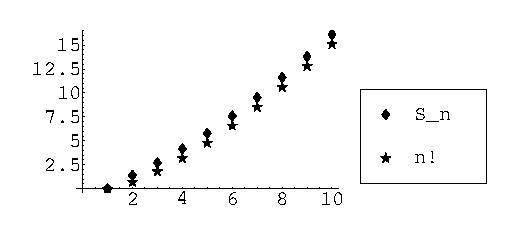
\includegraphics{Perms_gr1.eps}
\end{center}


The plot suggests that the ratio of $S_n$ and $n!$ converges to a constant, and a little experimentation, in lieu of analytical proof, reveals that constant to be $e=2.71828...$ In other words, as $n$ gets larger, $S_n$ approaches $e\times n!$, a convenient factoid.


Recall the imaginary dictionary containing an infinite number of alphabetically arranged subsections, each infinite in length. This dictionary was a mental image of the monoid of \emph{lists} of alphabetical characters, also known as the monoid of character strings under list concatenation.  Should we artificially limit the size of words in such a dictionary, we would no longer have a monoid, because the limited dictionary would not be closed under concatenation. But, we \emph{can} build a finite dictionary out of permutations. Such a dictionary would have the stupendous size $$1+S_{26}=1,096,259,850,353,149,530,222,034,277$$
ignoring differences between upper and lower case. This is a little larger than 1 billion billion billion. To set an intuition of the magnitude of this number, it is approximately the number of kilograms in the mass of the Earth. But it is finite.


Of course, this dictionary would suffer from the limitation that no duplicate letters would be permitted. This limitation is easily relieved, again in a finite fashion. Suppose we decide that words with more than four instances of a given letter are not interesting. Then, we can augment our alphabet, the type set $\T$, with three additional copies of each letter, artificially distinguished from one another by a subscript:
\[
 \{a,b,\ldots,z\}\rightarrow\{a_1,a_2,a_3,a_4,
 b_1,b_2,b_3,b_4,
 \ldots,z_1,z_2,z_3,z_4\}
\]
This device is just an application of \emph{disjoint union} from set theory. Now, our dictionary will have words with repeated letters, and will be of the more stupendous size:
\[
  1+S_{104}\approxeq 2.8\times 10^{166}
\]
which is approximately the square of the number of electrons in the observable Universe. So, while this new dictionary is technically finite, and is vastly smaller than Borges' library, it could never be physically written down, so, it is purely conceptual, once again.


The design of $\boxplus$ opens up can of worms of practical ramifications. A computer program implementing the operation for idempotent collection monoids must have a way of detecting whether a candidate element is already in a collection. The straightforward linear search --- iterating over the entire collection --- is only practical for small collections. Other search structures, like hash tables or B-trees, are a practical necessity in any scalable implementation.


The non-idempotent (infinite) collection monoids do not escape scot-free. If they are unordered, they must also have search optimizations, not for insertion, but for finding and grouping. Only lists can scalably perform both insertion and finding, at least finding-by-numerical-index, without search optimizations (though scalable finding requires array implementation with other ramifications on recursive programming patterns).


Let us round out the zoo of collection monoids with the following definitions:


\begin{definition}
  A \textbf{set} is an unordered, idempotent collection of zero or more items of some type $\T$. A monoid of sets has the associative, commutative, recursively idempotent, binary operation, $\cup$, for combining sets, and the empty set, $\{\}=\emptyset$, for identity.
\end{definition}


Just as a monoid of permutations can be finite, so can a monoid of sets. Again, suppose a base type set $\T$ with $n$ elements. The number of elements of a set monoid drawn from $\T$ is the sum of the number of sets of length $m$ for all $m\geq 0$ to $m\leq n$. The number of sets of length $m$ turns out to be
\[
  \frac{n!}{(n-m)! m!}\defeq \binom{n}{m}
\]
which is the binomial coefficient for $n$ and $m$. This is the same as the number of permutations of length $m$ divided by $m!$ because now, the order does not matter, and there are $m!$ different ways to rearrange the elements of a permutation of length $m$. The sum of the number of sets for all $m$ is the same as the binomial $(x+y)^n$ evaluated at $x=1, y=1$. This is
\begin{align*}
  \sum_{m=0}^{n}\frac{n!}{(n-m)! m!}
  &=\binom{n}{0}+\binom{n}{1}+\cdots+\binom{n}{n-1}+\binom{n}{n}\\
  {}&{}\\
  =(x+y)^n\vert_{x=1,y=1}&=2^n
\end{align*}
Another way of seeing the result is that each set in the monoid is the result of independently choosing whether to include each element of $\T$. Since for each element of $\T$, there are two independent choices --- to include or not --- and there are $n$ elements of $\T$, there must be exactly $2^n$ sets. The monoid is just the \emph{power set} of $\T$, that is, the set of all subsets of $\T$.


To relate this to databases, consider a set of employees:
\begin{center}
\begin{tabular}{l}
  \verb"John Smith"\\
  \verb"Jean Green"\\
  \verb"Joe Snow"
\end{tabular}
\end{center}
Think of this set as a type set, $\T$, and think of the monoid of sets drawn from this type set. This monoid would be the collection of all subsets of $\T$ --- the power set of $\T$, and would have eight elements. Its monoid combination operation would be set union, $\cup$. The next section of this tutorial exhibits transformations from such a monoid to others, and how such transformations effect various `database queries' over this table of employees.


We might examine the idea of a `dictionary' built from sets of characters, just as we did for lists and permutations, but this would be a boring one, since for every choice of characters, no matter what their order, there would be only one entry. Since the essence of words built of characters is order, the monoid of sets of characters would hardly rate the moniker `dictionary.'


\begin{definition}
  A \textbf{bag} or \textbf{multiset} is an unordered collection of zero or more items of some type $\T$. A monoid of bags has the associative, commutative, non-idempotent, binary operation, $\uplus$, for combining bags, and the empty bag, $\emptybag$, for identity.
\end{definition}


A bag is like a list, except that order does not matter. So, $\LBag 1, 1, 2, 3 \RBag$ is the same as $\LBag 2, 1, 3, 1\RBag$ and the same as all twenty-two other arrangements of 1, 1, 2, and 3. Just as with lists, there are no finite bag monoids other than the trivial bag monoid, which contains only the empty bag. Just as with lists, the reason is that from any two bags, we can form a larger bag by merging the two \emph{via} the bag-combination operation, $\uplus$.


\begin{observation}
All non-idempotent collection monoids are infinite.
\end{observation}


In the database context, \emph{bag} is the default type, because databases permit duplicates. So, a table of employees, without further conditioning, might look like this:
\begin{center}
\begin{tabular}{l}
  \verb"John Smith"\\
  \verb"Jean Green"\\
  \verb"John Smith"\\
  \verb"Joe Snow"
\end{tabular}
\end{center}
This table is obviously not the full monoid of bags of such names --- such a monoid is infinite. It is just a particular element of the monoid --- a particular bag of those names.


The two copies of \verb"John Smith" are most probably not an error. It would not be surprising to have two employees with the same name, but it is incumbent on the database designer to do something to distinguish them. The usual thing is to add a column containing an arbitrary but unique employee number for each employee, and then to set a \emph{database constraint} declaring that number to be a \emph{primary key} in the table. This is an operational constraint that must be maintained at run time, incurring computational cost, as discussed above. It effectively transforms the \emph{bag} of employees to a \emph{set} of employees through a device equivalent to the disjoint union, also discussed above. There is much more about such transformations in the next section of this tutorial, but, suffice it to say, while \emph{bag} is the default in databases, \emph{set} is quite often the desired behavior.


\subsection{\color{red}Summary}


The following tables summarize everything established so far and submits a few more non-collection samples for your consideration ($\mathbb{Z}$ is the set of all integers, positive, negative, and zero; in the last column of the second table, C and I stand for commutative and idempotent, respectively). While perusing the tables, remember that, especially in the case of the collection monoids, the interpretation of the definition of a monoid, ``$\Mon{\T}{\oplus}{\Z}$ \ldots a set of elements of type $\T$ \ldots'', must include subjecting the elements of $\T$ to the unit function to bring them into the monoid as singletons.


\begin{center}
\begin{tabular}{|l|l|}
  \hline
  $\Mon{\nats}{+}{0}$ & Natural numbers under addition only \\ \hline
  $\Mon{\nats}{\times}{1}$ & Natural numbers under multiplication only \\ \hline
  $\Mon{\nats}{\max_{\nats}}{0}$ & Natural numbers with a binary \emph{max} operation \\ \hline
  $\Mon{\nats\cup\{\infty\}}{\min_{\nats}}{\infty}$ & Natural numbers and Infinity with a binary \emph{min} operation \\ \hline
  $\Mon{\ints\cup\{-\infty\}}{\max_{\ints}}{-\infty}$ & All whole numbers and
  --Infinity \& binary \emph{max} operation \\ \hline
  $\Mon{\ints\cup\{\infty\}}{\min_{\ints}}{\infty}$ & All whole numbers and
  Infinity \& binary \emph{min} operation \\ \hline
  $\Mon{\mathrm{bool}}{\lor}{\mathrm{false}}$ &
  The set $\mathrm{bool}=\{\mathrm{true},\mathrm{false}\}$ with logical \emph{or} operation, $\lor$\\ \hline
  $\Mon{\mathrm{bool}}{\land}{\mathrm{true}}$ &
  The set bool with logical \emph{and} operation, $\land$ \\ \hline
	\hline
  $\Mon{\T}{\pp}{\emptylist}$ & lists of elements that are of type $\T$ \\ \hline
  $\Mon{\T}{\boxplus}{\emptyperm}$ & permutations of elements that are of type $\T$ \\ \hline
  $\Mon{\T}{\cup}{\emptyset}$ & sets of elements that are of type $\T$ \\ \hline
  $\Mon{\T}{\uplus}{\emptybag}$ & bags of elements that are of type $\T$ \\ \hline
\end{tabular}
\end{center}


Notice that the operation, alone, suffices to identify each kind of monoid. In later sections, we may feel free to abbreviate the notation by saying, for instance, that $\boxplus$ denotes a monoid of permutations or that $\lor$ denotes the \emph{or} monoid.


\begin{center}
		\begin{tabular}{|l|l||c||c|c|c|}
		  \hline monoid &
		  singleton type   & $\oplus$        & $\Z$  & $U$         & C/I \\
		      \hline \hline
		  $\Mon{\nats}{+}{0}$ &
		  $\nats$     & $+$             & 0              &
		      $\mathrm{id}=\lambda x.x$                            & C  \\ \hline
		  $\Mon{\nats}{\times}{1}$ &
		  $\nats$     & $\times$        & 1              &
		      $\mathrm{id}$                                        & C  \\ \hline
		  $\Mon{\nats}{\max_{\nats}}{0}$ &
		  $\nats$                 & $\max_{\nats}$   & 0           &
		      $\mathrm{id}$                                        & CI \\ \hline
		  $\Mon{\nats\cup\{\infty\}}{\min_{\nats}}{\infty}$ &
		  $\nats\cup\{\infty\}$   & $\min_{\nats}$   & $\infty$    &
		      $\mathrm{id}$                                        & CI \\ \hline
		  $\Mon{\ints\cup\{-\infty\}}{\max_{\ints}}{-\infty}$ &
		  $\ints\cup\{-\infty\}$  & $\max_{\ints}$   & $-\infty$   &
		      $\mathrm{id}$                                        & CI \\ \hline
		  $\Mon{\ints\cup\{\infty\}}{\min_{\ints}}{\infty}$ &
		  $\ints\cup\{\infty\}$   & $\min_{\ints}$   & $\infty$    &
		      $\mathrm{id}$                                        & CI \\ \hline
		  $\Mon{\mathrm{bool}}{\lor}{\mathrm{false}}$ &
		  bool & $\lor$          & false    & $\mathrm{id}$ & CI \\ \hline
		  $\Mon{\mathrm{bool}}{\land}{\mathrm{true}}$ &
		  bool & $\land$         & true     & $\mathrm{id}$ & CI \\ \hline
		  \hline
		  lists &
		  $[\T]$            & $\pp$      & $\emptylist$ &
		      $\lambda x.[x]$                        & neither \\ \hline
		  permutations &
		  $\LPerm \T\RPerm$ & $\boxplus$ & $\emptyperm$ &
		      $\lambda x.\LPerm x\RPerm$ &I\\ \hline
		  sets &
		  $\{\T\}$          & $\cup$     & $\{\}=\emptyset$  &
		      $\lambda x.\{x\}$                      & CI \\ \hline
		  bags &
		  $\LBag \T\RBag$   & $\uplus$   & $\emptybag$  &
		      $\lambda x.\LBag x\RBag$               & C\\ \hline
		\end{tabular}
\end{center}


Here is another table that categorizes the kinds of collection monoids, making it obvious why there are just four kinds:


\begin{center}
  \begin{tabular}{|l||c|c|}
  \hline
  \mbox{}       & \textbf{idempotent} & \textbf{not idempotent}  \\ \hline \hline
  \multirow{2}{*}{\textbf{commutative}}
                           & set               & bag             \\
  \mbox{}                  & $\{\T\}$          & $\LBag \T\RBag$ \\ \hline
  \multirow{2}{*}{\textbf{not commutative}}
                           & permutation       & list            \\
  \mbox{}                  & $\LPerm \T\RPerm$ & $[\T]$          \\ \hline
  \end{tabular}
\end{center}


Another effective way to look at this information is as follows:
\[
\xymatrix
{
                                   & bag\ar[dr]^{idem}  &     \\
  list\ar[ur]^{comm}\ar[dr]_{idem} &                    & set \\
                                   & perm\ar[ur]_{comm} &     \\
}
\]


\emph{List} is the most primitive kind of collection monoid, because it has neither of the qualifications of commutativity (order-independence) or idempotency (lack of duplicates). Add commutativity to a list monoid, and get a bag monoid. Add idempotency to a bag monoid, get a set monoid. Add idempotency to a list monoid, get a permutation monoid. Add commutativity to a permutation monoid, get a set monoid. Add both commutativity and idempotency to a list monoid, by either pathway, get a set monoid.


And the final way to look at it is to say the two kinds of commutative collection monoid are \emph{set} and \emph{bag} and the two kinds of idempotent collection monoid are \emph{set} and \emph{permutation}.


As another abbreviation, it can be convenient to denote the types or kinds of collection monoids using just the type symbols for their singleton elements, namely $[\T]$, $\pmx{\T}$, $\{\T\}$, and $\LBag\T\RBag$, and to write $(\T)$ to be a generic catch-all symbol meaning any of the four kinds of collection monoid. This abbreviation does run the risk of confounding the type of a collection monoid with the type of the subset containing just singleton members, but at this point, we hope the distinction is so familiar that the overloading of the type symbol does not cause heartburn. We feel free to use these abbreviations in the sequel.

\section{\color{Red}Mapping One Monoid to Another}


Once we figure out how to convert elements of one monoid to elements of another, we have everything we need for all kinds of queries. The queries familiar from relational databases \emph{are} nothing more nor less than transformations from one monoid to another. Think of a query that gets a list of distinct salaries from an employee database. Database practitioners will recognize this as
\begin{center}
  \begin{verbatim}
    SELECT DISTINCT e.salary
    FROM employees e
  \end{verbatim}
\end{center}
and we will recognize it as transformation from a collection monoid of employees to a monoid of sets of salaries. Given \emph{any} particular collection of employees --- an element of a collection monoid of employees, the transformation will return the correct set of salaries --- an element of a monoid of sets of salaries. If we had left off the \verb"DISTINCT", we would have gotten an element of a monoid of \emph{bags} of salaries, and the statement above would have been a transformation from a collection monoid of employees to a monoid of bags of salaries. 


In the following, we show how to construct arbitrary monoid-to-monoid transformations, and argue, by example, that any query one would care to make over database tables, over XML streams, or over structured graphs of objects in memory is such a transformation. 


Let $\M{1}=\Mon{\T}{\oplus_{1}}{\Z_{1}}$ and $\M{2}=\Mon{\Sb}{\oplus_{2}}{\Z_{2}}$ be two monoids. 
\begin{definition}
A \textbf{monoid homomorphism} is a transformation from $\M{1}$ to $\M{2}$ --- a prescription for converting elements of $\M{1}$ to elements of $\M{2}$ --- that preserves the monoid operations. 
\label{def:monoidhomomorphism}
\end{definition}
The rest of this section explains this definition. Note the following fine points:
\begin{enumerate}
  \item A \textbf{mapping} is a generic prescription for converting inputs, drawn from a \textbf{domain} set, to outputs, elements of a \textbf{range} or \textbf{codomain} set. A mapping may not have an output defined for every conceivable input, and it may have more than one output defined for some particular inputs.
	\item A \textbf{partial function} is a mapping that does not have an output for every input, but has a single output when it has any output.
	\item A \textbf{function} is a mapping that has a single output value for every input value in its domain. A function \textbf{covers} its domain. The fact may be emphasized by calling it a \textbf{total function}.
	\item A \textbf{surjection} is a function that covers the codomain, meaning that for every value in the codomain there is at least one element of the domain that maps to it. Synonyms are \textbf{surjective function} or \textbf{onto function}, with the word `onto' being abused as an adjective. 
	\item An \textbf{injection} is a function with the property that any particular output value corresponds to at most one input value. Synonyms are \textbf{injective function} or \textbf{one-to-one function}. 
  \item A \textbf{bijection} or a \textbf{one-to-one correspondence} is a function that is both an injection and a surjection. 
	\item A \textbf{multi-valued function} or \textbf{non-deterministic function} is a mapping that has more than one output for at least one particular input. It is not a function, so the English, here, is contradictory. But this is the standard nomenclature. 
	\item The inverse of a surjection is either a multi-valued injection or an injection.
	\item The inverse of an injection is either a partial surjection or a surjection.
	\item The inverse of a bijection is a bijection. 
	\item An \textbf{isomorphism} is a bijection that preserves all operations and structure. The domain and codomain of an isomorphism are \textbf{isomorphic}. For all intents and purposes, isomorphic sets are identical.
	\item A \textbf{transformation} is a total function with some additional proviso. In the case of monoid homomorphisms, the proviso is `preserving the monoid operations.'
\end{enumerate}


Start off with a concrete example: let $\M{1}$ be $\Mon{\T}{\pp}{\emptylist}$, the monoid of lists of elements of any type $\T$, and $\M{2}$ be $\Mon{\nats}{+}{0}$, the monoid of integers under addition. Let $c$ be the particular homomorphism that counts the number of members of a list, defined recursively as follows:
\begin{align*}
  c(\emptylist)        & = 0 \\
  c([x]\pp\mathcal{L}) & = 1 + c(\mathcal{L})
\end{align*}
where $[x]$ is a singleton list and $\mathcal{L}$ is any list in $\M{1}$. It is clear that $c$ has $\M{1}$ covered, meaning that no matter what list from $\M{1}$ you give to $c$, it will give an answer. It is also clear that every application of $c$ will yield just one answer, so $c$ is, indeed, a function from $\M{1}$ to $\M{2}$. 

The most important thing to note is how $\pp$ operations in $\M{1}$ become $+$ operations in $\M{2}$. The homomorphism, $c$, not only converts elements of $\M{1}$ to elements of $\M{2}$, but converts the \emph{operation} of $\M{1}$, in parallel, to the \emph{operation} of $\M{2}$. Thus, $c$, while it is a function, is not \emph{just} a function, but a transformation. The mapping of operations holds not just for singletons, but for arbitrary lists in $\M{1}$ Let us deduce, from the above, that 
\begin{equation}
  c(\mathcal{L}_{1}\pp\mathcal{L}_{2})=c(\mathcal{L}_{1})+c(\mathcal{L}_{2})
  \label{eqn:inducl}
\end{equation}
where $\mathcal{L}_{1}$ and $\mathcal{L}_{2}$ are any lists whatever. How? By induction. The next paragraph covers the argument in detail. However, this kind of argument follows such a clear and frequent pattern that, in the rest of this tutorial, we simply say ``by induction'' and assume the point made. 


Equation \ref{eqn:inducl} is certainly true when $\mathcal{L}_{1}$ is a singleton, by the definition of $c$, or when $\mathcal{L}_{1}$ is the empty list, which is the identity of the list monoid, so that
\begin{align*}
  c(\emptylist\pp\mathcal{L}_{2})&=c(\mathcal{L}_{2})\\
  =0+c(\mathcal{L}_{2})&=c(\emptylist)+c(\mathcal{L}_{2})
\end{align*}
The only remaining case is where $\mathcal{L}_{1}$ has more than one element. Write it as $[x]\pp\mathcal{L}_{0}$, with $\mathcal{L}_{0}$ arbitrary non-empty.\footnote{The argument is stronger than necessary: we could allow $\mathcal{L}_{0}$ to be empty, but it is perhaps more clear this way.} The definition of $c$ guarantees that $c(\mathcal{L}_{1})=1+c(\mathcal{L}_{0})$. Assume, hypothetically (for the sake of argument), that 
$$c(\mathcal{L}_{0}\pp\mathcal{L}_{2})=c(\mathcal{L}_{0})+c(\mathcal{L}_{2})$$
Now consider 
$$\mathcal{L}_{1}\pp\mathcal{L}_{2}=[x]\pp\mathcal{L}_{0}\pp\mathcal{L}_{2}$$
By associativity, which holds for any monoid operation, write 
\begin{align*}
  c([x]\pp(\mathcal{L}_{0}\pp\mathcal{L}_{2})) &=
  1+c(\mathcal{L}_{0}\pp\mathcal{L}_{2})\\
  &= 1+c(\mathcal{L}_{0})+c(\mathcal{L}_{2})\\
  &= c(\mathcal{L}_{1})+c(\mathcal{L}_{2})  \\
  =c(([x]\pp\mathcal{L}_{0})\pp\mathcal{L}_{2})
  &=c(\mathcal{L}_{1}\pp\mathcal{L}_{2})
\end{align*} 
We have proved equation \ref{eqn:inducl} for the empty and singleton cases, and we have proved that \emph{if} it is true for a list of any length \emph{then} it is true for a list of length one greater. Therefore it must be true for lists of any length. $\blacksquare$


Generalizing, for $\phi$ to be a transformation from $\M{1}$ to $\M{2}$ means that $\phi(a_1)=a_2$ and $\phi(b_1)=b_2$ are definite elements of $\M{2}$ just when $a_1$ and $b_1$ are elements of $\M{1}$ because the transformation is a function with a proviso. The proviso is `preserve the monoid operations,' but what does that mean in general? It has to be that usage of $\oplus_1$ gets turned into usage of $\oplus_2$ roughly as follows:
\begin{equation}
  \phi(a_1 \oplus_1 b_1) = \phi(a_1) \oplus_2 \phi(b_1) = a_2 \oplus_2 b_2
  \label{eqn:homomorphismOne}
\end{equation}
but this causes a problem. Suppose $\M{1}$ is an idempotent monoid, meaning that 
$$a_1 \oplus_1 a_1 = a_1$$
Then, the attempt at preserving operations, equation \ref{eqn:homomorphismOne}, implies that
$$\phi(a_1 \oplus_1 a_1) = \phi(a_1)\oplus_2\phi(a_1)=a_2\oplus_2 a_2$$
but also that
$$\phi(a_1 \oplus_1 a_1) = \phi(a_1)= a_2$$


All is well if $\M{2}$ is also idempotent, but, if not, then $a_2\oplus_2 a_2=a_2$ could be wrong, and this calculation could lead to a contradiction. In particular, this makes it impossible to count the number of members in a set with a monoid homomorphism:
\begin{align*}
  \phi\left(\{a\}\cup\{a\}\right)&=\phi\left(\{a\}\right)+\phi\left(\{a\}\right)=2\\
  \phi\left(\{a\}\cup\{a\}\right)&=\phi\left(\{a\}\right)=1
\end{align*}


We must introduce an auxiliary binary operation of \emph{difference} or \emph{minus}. This operation is not allowed within the monoid, but prevents duplicate operations when mapping idempotent monoids to non-idempotent ones. Let us develop \emph{minus} by comparison to set union. The monoid operation for sets is $\cup$ or \emph{union}, not formally defined up to this point; let us do that here:
\begin{definition}
  If $A$ and $B$ are sets, then $A\cup B$, read ``$A$ \emph{union} $B$,'' is the set of elements that appear either in $A$ or $B$.
\end{definition}
So, $\{1,2\} \cup \{2,3\}=\{1,2,3\}$, for instance.


Now, given two sets, here is their difference
\begin{definition}
  If $A$ and $B$ are sets, then $A-B$, read ``$A$ \emph{minus} $B$,'' is the set of elements that appear in $A$ and not in $B$.
\end{definition}
So, $\{1,2\} - \{2,3\}=\{1\}$. This sort of definition works for the other idempotent monoid, permutations, because the order in which one takes elements out of a permutation does not matter. 
\begin{equation*}
  \pmx{1,2,3}-\pmx{3,2} = \pmx{1,2,3}-\pmx{2,3}
\end{equation*}


\begin{definition}
  If $A$ and $B$ are permutations, then $A-B$, read ``$A$ \emph{minus} $B$,'' is a permutation consisting of the elements in $A$, but not in $B$, without changing the order in $A$.
\end{definition}


We are now equipped, with \emph{minus} defined for both kinds of idempotent monoids, to resolve the conundrum by writing


\begin{definition} A monoid homomorphism $\phi : \M{1}\rightarrow\M{2}$ (definition \ref{def:monoidhomomorphism}) \textbf{preserves the monoid operations} through the following device:
\begin{equation}
  \phi(a \oplus_1 b) = \phi(a)\oplus_2\psi(\phi,b,a)
\end{equation}
where
\begin{equation}
  \psi(\phi,b,a)=
  \begin{cases}
    \phi(b-a) & \text{if $\M{1}$ is idempotent} \\ 
    \phi(b)   & \text{otherwise}
  \end{cases}
\end{equation}
\end{definition}
$\blacksquare$


Redoing the problematic computation of set length, it will no longer give out the pesky $2$:
\begin{align*}
  \phi\left(\{a\}\cup\{a\}\right) 
  &= \phi\left(\{a\}\right)+\psi\left(\phi,\{a\},\{a\}\right)\\
  &= \phi\left(\{a\}\right)+\phi\left(\{a\}-\{a\}\right) \\
  &= 1 + \phi\left(\emptyset\right)=1+0=1
\end{align*}


We \emph{could} have made this definition ever-so-slightly smaller by simply defining \emph{minus} to be \emph{no-operation} or \emph{nop} for non-idempotent monoids. But the definition is more clear as stated above. Sometimes, clarity trades off against conciseness; usually they work together. 


The similar problem of converting elements of a commutative (unordered) monoid into elements of a non-commutative (ordered) one is harder. Consider converting the set ${1,2,3}$ into a list. Can such a mapping be a homomorphism? Does it result in $[1,2,3]$ or $[2,1,3]$? What about the other four possible orders of $1$, $2$, and $3$? Since, without further information, the mapping does not have a unique result, it is not a properly defined function --- it is \emph{non-deterministic}. So it fails the first criterion for being a homomorphism, that of being a function, yielding a single output for every input. In this case, it is better to solve the problem in the particular, when it arises, than to attempt a general definition. So, we conclude:


\begin{observation}
Homomorphisms, in general, from commutative (unordered) collection monoids to non-commutative (ordered) collection monoids, do not exist.
\end{observation}


A natural question is whether the identity element of the source monoid always corresponds to the identity element of the destination monoid under any homomorphism. The answer is that it must, for, suppose it did not. Then, 
\[
  \phi(\mathcal{Z}_{1}) = x_2 \neq \mathcal{Z}_{2}
\]
would be some non-identity element. Now, pick some $m_1$ in $\mathcal{M}_1$ and consider the following calculation, which can lead to a contradiction:
\begin{align*}
  m_1 \oplus_1 \mathcal{Z}_1       &= m_1                   \\
  \phi(m_1 \oplus_1 \mathcal{Z}_1) &= \phi(m_1) \defeq m_2  \\
  {} &= \phi(m_1) \oplus_2 \psi(\phi,\mathcal{Z}_1,m_1) \\
  {} &= m_2 \oplus_2 x_2 \neq m_2 \text{ in general}
\end{align*}
\begin{lemma}
  A monoid homomorphism preserves the identity element.
\end{lemma}


\subsection{\color{red}A Zoo of Homomorphisms}


Consider the following idioms --- \emph{map}, \emph{filter}, and \emph{fold} --- from functional programming and their relationships with monoid homomorphisms. Let $\mathcal{A}\langle\T\rangle=(a_1,a_2,\ldots)$ be a representative element of any of the four kinds of collection monoid, with $a_{i}$ its constituent elements of type $\T$, $\Ux{A}=\Ux{()}$ its unit function, $\oplus$ its monoid operation, and $\Z$ its identity. Write the type of $\mathcal{A}\langle\T\rangle$ itself as $(\T)$. 


\subsubsection{\color{red}The \emph{map} idiom}


\emph{Map} is a function of two arguments. The first argument is another function, $f$, that converts elements $t$ of type $\T$ to elements, $s=f(t)$, of another type set, $\Sb$. The second argument of map is an element of a collection monoid, say $\mathcal{A}\langle\T\rangle$. The final output is an element of the same kind of collection monoid, but with a potentially different type set. Here is \emph{map}, operating on $\mathcal{A}\langle\T\rangle$:
\[
  \mathtt{map}\;f\;\mathcal{A}\langle\T\rangle= 
  \mathtt{map}\;f\;(a_1,a_2,\ldots) = 
  \left( f(a_1),f(a_2),\ldots\right) = \mathcal{A}\langle\Sb\rangle
\]
This does not change the kind of collection monoid to which $\mathcal{A}$ belongs, just the base type of the monoid's elements' elements, and, therefore, implicitly, the unit function that converts base-type elements to singletons in the monoid. 

We might say that if we feed \emph{map} its first argument only, that this combination, written $\mathtt{map}\;f$, is a function from $\mathcal{A}\langle\T\rangle$ to $\mathcal{A}\langle\Sb\rangle$, \emph{i.e.}, a function that converts elements of a collection monoid with base type $\T$ to elements of the same kind of collection monoid with base type switched out to $\Sb$. Write the type of this new combination function as follows:
\[
  \mathtt{map}\;f:\Mon{\T}{\oplus}{\Z}
    \rightarrow\Mon{\Sb}{\oplus}{\Z}
\]
There it is: the monoid homomorphism is $\mathtt{map}\;f$. It \emph{preserves} the monoid operation because it does not \emph{change} the monoid operation. The identity element of the two collection monoids is the same because it pertains to the monoid rather than to the base sets, $\T$ and $\Sb$. The unit function also pertains to the monoid, so doesn't change in any meaningful way. 

%Its domain and codomain change, but its functional action doesn't. Abbreviate $\Ux{()}$ as just $\U$ in the following:
%\begin{center}
%\begin{tabular}{ll}
%  $\U:\T\rightarrow(\T)$ & {\emph{$\U$ maps elements of $\T$ to singleton members of $(\T)=\Mon{\T}{\oplus}{()}$}}\\
%{$\rightarrow$}&{}\\
%  $\U:\Sb\rightarrow(\Sb)$ & {\emph{$\U$ maps elements of $\Sb$ to singleton members of $(\Sb)=\Mon{\Sb}{\oplus}{()}$}}\\
%\end{tabular}
%\end{center}

To derive a recursive form of the definition, we begin with a base case:
\begin{equation}
  \mathtt{map}\;f\;\emptycollection\defeq\emptycollection
\end{equation}
In other words, map has no effect on the empty collection. For the non-base case, as discussed at length concerning permutations, we apply a \emph{deconstruction rule} to the monoid-element argument:
\begin{align}
  \mathtt{map}\;f\;\mathcal{A}\langle\T\rangle
     &=\mathtt{map}\;f\;(a_1,a_2,\ldots)\nonumber\\
  {} &= \mathtt{map}\;f\;\left\lgroup (a_1)\oplus(a_2,\ldots)\right\rgroup 
         \nonumber\\
  {} &= \mathtt{map}\;f\;\left\lgroup \U(a_1)\oplus(a_2,\ldots)\right\rgroup
         \nonumber\\
  {} &= \mathtt{map}\;f\;\left\lgroup
     \U\left(a_1\right)\oplus{\mathcal{A}'\langle\T\rangle}
     \right\rgroup \nonumber\\
  {} &\defeq\U\left\lgroup
     f\circ\U^{-1}\left(
     \U\left(a_1\right)\right)\right\rgroup\oplus
     \left\lgroup\mathtt{map}\;f\;{\mathcal{A}'\langle\T\rangle}\right\rgroup
     \label{def:mapdefone}\\
  {} &\defeq\U\left(f\left(a_1\right)\right)\oplus
     \left\lgroup\mathtt{map}\;f\;{\mathcal{A}'\langle\T\rangle}\right\rgroup
     \label{def:mapdeftwo}
\end{align}
where $\mathcal{A}=(a_1)\oplus\mathcal{A}'$. There is quite a bit of subtle `junk' math going on, here, with the unit function, just to get consituent elements of $\mathcal{A}$ out of the collection monoid so $f$ can operate on them, then subjected to the unit again so they can get $\oplus$'ed back on to the front of the recursive application of $\mathtt{map}\;f$ to $\mathcal{A}'$. In the definition \ref{def:mapdefone}, the notation $f\circ\U^{-1}$ means \emph{function composition}, introduced at length below under the \emph{fold} idiom. In this case, \emph{map} composes $f$ with the \emph{inverse} of $\U$, written $\U^{-1}$. \emph{Map} may need to know how to \emph{decondition} singletons with the inverse of the unit function, to take them out of their collection monoid. We know from the preliminary points of this section that not every function has an inverse that is, itself, a function. Fortunately, the unit functions of all the kinds of colletion monoids are invertible. Such is \emph{not} the case for unit functions of non-collection monoids --- those may have multi-valued inverses. It turns out that, when used under \emph{map} as above, any value of a multi-valued inverse may be taken since the unit is immediately applied, a fact reflected in the second, alternative definition \ref{def:mapdeftwo}.


Keep these remarks in mind as we proceed through the \emph{filter} and \emph{fold} idioms, and as we endeavor to extend each of the idioms to non-collection monoids. Ultimately, these considerations will lead us to \emph{monads} over \emph{monoids}, since monads provide a clean, general technique for finessing away `junk' math over the unit functions. 


Here is an example of \emph{map} at work in a Haskell-like programming language. Suppose a function, $\mathtt{intToChar}$, which converts integers to their ASCII character equivalents. Now, suppose a list of integers, $[97, 98, 99]$. Convert the entire list of integers to their character equivalents as follows:
\begin{center}
  \verb"map intToChar [97,98,99]" $\rightarrow$ \verb$['a','b','c']="abc"$
\end{center}
So, \verb"map intToChar" will convert any list of integers --- any element of the monoid of lists of integers --- to a list of characters --- an element of the monoid of lists of characters. The final equality obtains because functional programming languages usually represent character strings as lists of individual characters.


The definition of \emph{map} also works for idempotent collection monoids like set. Suppose a function \verb"nextPrime" that maps integers to the next higher prime number, and map it over a set of integers, for instance, $1{\dotdot}10=\{1,2,\ldots10\}$ (in general, abbreviate the set of integers from $m$ to $n$ with double dots, as $\{ m{\dotdot}n\}$): 
\begin{center}
  \verb"map nextPrime {1..10}" $\rightarrow$ \verb"{2,3,5,7,11}" 
\end{center}
By this application, a set containing ten members becomes a set containing five members, because the duplicates get eliminated. In mathematics, elimination of duplicates is automatic, effortless, and almost magical. In real-world computation, we humans must do some work to program a computer to do some more work to get rid of them. 


Back to the generalities, write the type of the function $f$ as $\T\rightarrow\Sb$, and the type of \emph{map}, itself as something that transforms a function of type $\T\rightarrow\Sb$ to something of type $\Mon{\T}{\oplus}{\Z}\rightarrow\Mon{\Sb}{\oplus}{\Z}$:
\begin{equation}
  \mathtt{map}:(\T\rightarrow\Sb)\rightarrow
    \left(\Mon{\T}{\oplus}{\Z}
    \rightarrow\Mon{\Sb}{\oplus}{\Z}\right)
  \label{eqn:mapdefinition}
\end{equation}
So, \emph{map} is a \emph{homomorphism-maker}: feed it a function that transforms the base types, and \emph{map} gives you back a homomorphism amongst collection monoids.


\begin{remark}
Generally, given a function of multiple arguments, the idea of giving it its arguments one at a time and interpreting the results as functions of the remaining arguments is \emph{Currying}. A Curried function is a function of one argument that returns, recursively, a function of any remaining arguments. Any function can be Curried. To Curry a function of no arguments, just give it an argument to ignore. The similarity to the construction of collection monoids from singletons is intentional: Currying builds up multi-ary functions from unary functions, that is, from functions of single arguments.
\end{remark}


The \emph{map} idiom, as understood so far, produces homomorphisms for collection monoids. Can it be given any meaning for non-collection monoids? Let $\mathcal{L}_{\nats}$ be $\Mon{\nats}{+}{0}$ and $\mathcal{L}_{\ints}$ be $\Mon{\ints}{+}{0}$, and let $f$ be a function from $\nats$ to $\ints$ that, say, takes every input and returns its negative. So, $f(3)=-3$ and so on. $f$ is properly formed to be an argument of \emph{map} because $f$ is a function from the base-type set of a monoid to another base-type set of the `same kind of' monoid. What could be the meaning of $\mathtt{map}\;f$ in this case? How about a mapping from $\mathcal{L}_{\nats}$ to $\mathcal{L}_{\ints}$ that preserves the operation $+$? In other words, as a monoid homomorphism? Viewed this way, map fulfills exactly definition \ref{eqn:mapdefinition}. Specifically, it takes a function between two bare sets, namely $f$, and converts it into a homomorphism, namely $\mathtt{map}\;f$, between two instances of the same kind of monoid. The `kind' of monoid is specified by the monoid operation and the identity element, precisely what $\nats$ and $\ints$ have in common in our example. In this case, the homomorphism is not `onto' because it never produces a positive element of $\ints$. If we want an `onto' homomorphism, then we could view the target as the monoid of negative integers, $\mathcal{L}_{-\nats}$, which is certainly closed under addition and therefore a properly defined monoid. 


Now, recall that \emph{map} does some subtle juggling of the unit functions and their inverses. Let's look at a non-collection monoid like $\Mon{\nats}{+_{12}}{12}$ whose unit function has a multi-valued, non-functional inverse. That unit function is \emph{residual modulo 12}, and its inverse is multi-valued because, for instance, 1, 13, 25, \ldots are all preimages of 1. Therefore the `inverse' of 1 does not have a single answer, so it's not a function. Now, consider an $f$ like $\lambda x.x^2$, the function that just computes the square of its input. How could we compute, say, $\mathtt{map}\;(\lambda x.x^2)\;(7)_{12}$, where the monoid is the clock-arithmetic monoid? Well, since we immediately un-invert the inverse (see definitions \ref{def:mapdefone} and \ref{def:mapdeftwo}), we can pick \emph{any} of its values, because, in all cases, the answer is just $49$ mod $12=1$. 


All This means that we can promote the \emph{map} idiom from its origin over lists in functional programming up to general collection monoids and further up to non-collection monoids. 


\subsubsection{\color{red}The \emph{filter} idiom}


\emph{Filter} is a function of two arguments: (1) a predicate that, for any element of the type set $\T$, returns a boolean $\in\{\text{true},\text{false}\}$; and (2), an element of a collection monoid $\mathcal{A}=\Mon{\T}{\oplus}{\Z}$ of type $(\T)$. It is defined as follows:
  $$\mathtt{filter}\;p\;\mathcal{A}=\bigoplus^n_{i=1}
    \begin{cases}
       \U(a_i) & \text{if $p(a_i)$} \\ 
       \Z & \text{otherwise}
    \end{cases}$$
This just means ``use $\oplus$ to combine either the singleton $\U(a_i)$ or the identity $\Z$ of the monoid into the overall result for every $a_i$ in the input, depending on whether the predicate $p(a_i)$ evaluates to true.'' An alternative definition, in recursive style, equivalent in every way for collection monoids, is the following:
  $$\mathtt{filter}\;p\;(a_1,a_2,\ldots,a_n) =
  \begin{cases}
    \U(a_1)\oplus\mathtt{filter}\;p\;(a_2,\ldots,a_n) & \text{if $p(a_i)$} \\
    \mathtt{filter}\;p\;(a_2,\ldots,a_n) & \text{otherwise}
  \end{cases}$$

Following in the footsteps of \emph{map}, above, consider these type expressions:
\begin{center}
\begin{tabular}{ll}
  $p:\T\rightarrow\{\text{true},\text{false}\}$ 
    & \parbox{2.85in}
      {\footnotesize\emph{The type of $p$ is `function from 
      $\T$ to the boolean constants'}}\\
  {}&{}\\
  $\mathcal{A}:(\T)$ 
    & \parbox{2.85in}
      {\footnotesize\emph{The type of $\mathcal{A}$ is $(\T)$ or 
      `collection monoid with base type $\T$'}}\\
  {}&{}\\
  $\mathtt{filter}\;p\;\mathcal{A}:(\T)$
    & \parbox{2.85in}
      {\footnotesize\emph{The type of $\mathtt{filter}\;p\;\mathcal{A}$ 
      is also $\T$}}\\
  {}&{}\\
  $\mathtt{filter}\;p:(\T)\rightarrow(\T)$
    & \parbox{2.85in}
      {\footnotesize\emph{The type of $\mathtt{filter}\;p$ is 
      $(\T)\rightarrow(\T)$, 
      or `function from $(\T)$ to $(\T)$,' that is, a monoid homomorphism}}\\
  {}&{}\\
  $\mathtt{filter}:(\T\rightarrow\{\text{true},\text{false}\})
    \rightarrow(\T)\rightarrow(\T)$
    & \parbox{2.85in}
      {\footnotesize\emph{The type of $\mathtt{filter}$ is `function 
      of a predicate that returns a monoid homomorphism'}}\\
\end{tabular}
\end{center}


So $\mathtt{filter}\;p$ is a homomorphism from $(\T)$ to $(\T)$, and \emph{filter} is another homomorphism-maker, this time, a function that converts \emph{predicates} into monoid homomorphisms. Each resulting homomorphism changes none of the the base type, the operation, the unit, or the identity of the monoid; it just removes elements from elements of the source collection monoid that happen not to satisfy the predicate $p$. 


So, how do the source and destination monoids differ? They may or may not. The most straightforward interpretation of homomorphism $\mathtt{filter}\;p$ is that it just takes an element of a monoid and produces another element of the same monoid. But, depending on one's point of view and details of the predicate, it also produces an element of another monoid, one in which elements of the base type --- constituents elements of the elements of the monoid --- are only those that satisfy $p$! Suppose $p$ is \emph{even?}, the predicate that returns \emph{true} if its argument is an even element of $\nats$ and \emph{false} otherwise, and the source monoid is lists of natural numbers, $[\nats]$. Then, $\mathtt{filter}\;p$ could be viewed either as a homomorphism to the distinct monoid of lists of even integers or as a homomorphism back to $[\nats]$, just one that happens always to produce lists of even numbers. 


This will work for predicate \emph{odd?}, too, since a set of \emph{collections} of odd numbers is a monoid. But, a set of odd numbers, under $+$, is not a monoid because it's not closed: the sum of two odd numbers is nod odd. So what sense can we make of \emph{filter} for non-collection monoids? Once again, let $\mathcal{L}_{\nats}$ be $\Mon{\nats}{+}{0}$. Recall that the unit function for this monoid is $\lambda x.x$, the identity function. Now, let $p$ be \emph{even?}. Looking at the development above, $\mathtt{filter}\;p$ could be a monoid homomorphism to the monoid of even natural numbers under $+$ with $0$ as identity element. That is a proper monoid, since the sum of any two even integers is an even integer. It would not work if the predicates were \emph{odd?} or \emph{prime?}, since the destinations would not be monoids (adding two primes does not necessarily produce a prime, and adding two odds never produces an odd). The lesson, here, is to be careful:


\begin{observation}
  $\mathtt{filter}\;p$ over non-collection monoids may produce outputs in a set that is not a monoid. 
\end{observation}


The predicate can depend upon any attributes of its input. \emph{Filter} creates a different homomorphism for each predicate. Imagine a predicate that can test an employee record for, say, green-card status: \[\mathtt{hasGreenCard}:
\text{employeeRecord}\rightarrow\text{bool}\]
Then, 
\begin{center}
\verb"filter hasGreenCard"
\end{center}
is a homomorphism that will take an element of any collection monoid of employee records and return an element of another collection monoid --- of the same kind of collection --- containing only those employees with green cards. This is just what the following SQL would do, presuming an attribute to store or method to compute the predicate:
\begin{center}
\begin{tabular}{l}
\verb"SELECT e"\\
\verb"FROM employees e"\\
\verb"WHERE e.hasGreenCard"
\end{tabular}
\end{center}


\subsubsection{\color{red}The \emph{fold} idiom}


So far, we have a way of building monoid homomorphisms that change the base type ($\mathtt{map}\;p$) and a way of building monoid homomorphisms that change the members of the monoid ($\mathtt{filter}\;p$) without changing the base type. This next idiom changes the kind of monoid but not the base type. Recall that $\mathcal{A}$ is an element of an arbitrary collection monoid, $\Mon{\T}{\oplus}{\Z}$. Abbreviate the monoid as $\Mx{A}$. Now, suppose another monoid, not necessarily a collection monoid $$\Mx{B}\defeq\Mon{\T}{\otimes}{\mathcal{Y}}$$
with unit function $\Ux{B}:\T\rightarrow\Mx{B}$. To make things easier to see, let
\begin{equation}
  b_i = \Ux{B}(a_i)
  \label{eqn:monadunit}
\end{equation}
The $b_i$ are singletons in the new monoid, $\Mx{B}$, brought in one at a time from the constituent elements $a_i\in\T$ of $\mathcal{A}\in\Mx{A}$. 


\emph{Fold} is a function of three arguments: (1) the monoid operation, $\otimes$, of $\Mx{B}$; (2) its corresponding monoid identity element, $\mathcal{Y}$; and (3) an element $\mathcal{A}$ of a source collection monoid, $\Mx{A}$, potentially of a different kind from $\Mx{B}$. Given its first two arguments, \emph{fold} converts its last argument into an element of the kind of monoid implied by its first two arguments. Define
\begin{equation}
    \mathtt{fold}\;\otimes\;\mathcal{Y}\;\mathcal{A} \defeq
        b_{1}\otimes
        (b_{2}\otimes
        (\ldots(b_{n}\otimes
        \mathit{\mathcal{Y}})\ldots))
  \label{eqn:folddef}
\end{equation}
or, more explicitly:
  $$ \mathtt{fold}\;\otimes\;\mathcal{Y}\;\mathcal{A} \defeq
        \Ux{B}(a_1)\otimes
        \left\lgroup
        \Ux{B}(a_2)\otimes
        \left\lgroup\ldots\left\lgroup
        \Ux{B}(a_n)\otimes
        \mathit{\mathcal{Y}}
        \right\rgroup\ldots\right\rgroup
        \right\rgroup $$


In recursive style, the base case is
\begin{equation}
  \mathtt{fold}\;\otimes\;\mathcal{Y}\;\emptycollection\defeq\mathcal{Y}
\end{equation}
and the rest is
\begin{equation}
  \mathtt{fold}\;\otimes\;\mathcal{Y}\;\mathcal{A} \defeq
    \Ux{B}(a_1)\otimes
    \left\lgroup
    \mathtt{fold}\;\otimes\;\mathcal{Y}\;\mathcal{A}'
    \right\rgroup
\end{equation}
where $\mathcal{A}=(a_1)\oplus\mathcal{A}'$. 


Notice that the unit function, $\Ux{B}$ is not one of the arguments of \emph{fold}. As before, the unit is just implied by the other attributes of the destination monoid $\Mon{\T}{\otimes}{\mathcal{Y}}$, in this case, by $\otimes$ and $\mathcal{Y}$.


So, $\mathtt{fold}\;\otimes\;\mathcal{Y}$ --- given just two of its three arguments, as we can always do because of Currying --- is a function that converts any instance of an input \emph{collection} monoid to an instance of another monoid, $\Mon{\T}{\otimes}{\mathcal{Y}}$, not necessarily a collection monoid. In other words, $\mathtt{fold}\;\otimes\;\mathcal{Y}$ is a monoid homomorphism. That means that \emph{fold} must be another homomorphism-maker. Just as we did with \emph{map} and \emph{filter} above, let us write out \emph{fold's} types:


\begin{center}
\begin{tabular}{ll}
  $\mathtt{fold}\;\otimes\;\mathcal{Y}:
    \Mx{A}\rightarrow\Mx{B}$
    & \parbox{2.85in}{\footnotesize\emph{The 
      type of $\mathtt{fold}\;\otimes\;\mathcal{Y}$
      is `function from $\Mon{\T}{\oplus}{\Z}$ to 
      $\Mon{\T}{\otimes}{\mathcal{Y}}$', or just $\Mx{A}\rightarrow
      \Mx{B}$ for short; that is, a homomorphism from 
      any collection monoid $\Mx{A}$
      to a monoid $\Mx{B}$}} \\
  {}&{}\\
  $\mathtt{fold}\;\otimes:\mathcal{Y}\rightarrow
    \Mx{A}\rightarrow\Mx{B}$
    & \parbox{2.85in}{\footnotesize\emph{The 
      type of $\mathtt{fold}\;\otimes$
      is `function from an identity element, $\mathcal{Y}$, to a
      homorphism from any monoid $\Mx{A}$
      to a monoid $\Mx{B}$'}}\\
  {}&{}\\
  $\mathtt{fold}:\otimes\rightarrow\mathcal{Y}\rightarrow
    \Mx{A}\rightarrow\Mx{B}$
    & \parbox{2.85in}{\footnotesize\emph{The 
      type of $\mathtt{fold}$
      is `function from an operation, $\otimes$ and a 
      identity element, $\mathcal{Y}$, to a
      homorphism from any monoid $\Mx{A}$
      to a monoid $\Mx{B}$'}}\\
  \end{tabular}
\end{center}


\emph{Fold} lets us, quite prettily, specify the target monoid homomorphism in bits and pieces. Fully specify it by writing $\mathtt{fold}\;\otimes\;\mathcal{Y}$; that expression is ready to take a monoid instance, $\mathcal{A}\in\Mx{A}$, and convert it into an instance $\mathcal{B}$ of $\Mx{B}$. Specify the target monoid's operation, but not its identity element, by writing $\mathtt{fold}\;\otimes$. Give that expression an identity element to get a monoid homomorphism. Delay all commitments by writing just $\mathtt{fold}$: to get a monoid homomorphism, supply both an operation and a identity element.


\emph{Fold} is extremely versatile. Recall that this section started off with a homomorphism, $c$, from lists of elements, $\Mon{\T}{\pp}{\emptylist}$, to the monoid of natural numbers under addition, $\Mon{\nats}{+}{0}$. That homomorphism effects a count of the number of elements in the list. We defined $c$ explicitly by its actions on the empty list and, recursively, its action on a list consisting of a singleton concatenated to another list. Can we get an equivalent homomorphism out of \emph{fold}? Easily. First, map a function that converts anything to the constant 1 over the list, then apply \verb"fold + 0" to the result. The result will be a member of $\Mon{\nats}{+}{0}$. 


Generalizing the above yields a prescription for \emph{function composition}. In general, if $g$ is a function from a set $A$ to a set $B$, and $f$ is a function from $B$ to a set $C$, then the composition of $f$ and $g$, written $f\circ g$, is the function from $A$ to $C$ defined by $f(g(a))$ for any $a$ in $A$. Spelling it out:
\begin{align*}
  g:\mathcal{A}\rightarrow\mathcal{B}\\
  f:\mathcal{B}\rightarrow\mathcal{C}\\
  f\circ g:\mathcal{A}\rightarrow\mathcal{C}
\end{align*}


The function to map over the lists is $\lambda x.1$, and $$g\defeq\mathtt{map}\;\lambda x.1:[\T]\rightarrow[1]$$ is a homomorphism from a list monoid of elements of any type to the (unique) monoid of lists of copies of the natural number 1. This homomorphism preserves the number of elements in the list, as would any map over a list, but changes every input element into the number 1. Now, let $f$ be \verb"fold + 0", the homomorphism that takes any collection of natural numbers and sums them. The composition
\[  
  c=f\circ g= (\mathtt{fold}\;+\;0) \circ (\mathtt{map}\;\lambda x.1)  
\]
will be the monoid homomorphism that counts the elements in any list. 


What meaning can \emph{fold} have if its third argument is not a collection monoid? Note that $\mathcal{A}$, an element of the monoid $\Mx{A}$, will have a constituent element $a$ such that  $\mathcal{A}=\Ux{A}(a)$. The definition of \emph{fold} in equation \ref{eqn:folddef} now leads us to write
\begin{equation}
  \mathtt{fold}\;\otimes\;\mathcal{Y}\;\mathcal{A} \defeq
        \Ux{B}(a)=
        \Ux{B}\left({\mathcal{U}}^{-1}_{\mathcal{A}}
        \left(\mathcal{A}\right)\right)
  \label{eqn:foldnoncollectiondef}
\end{equation}
So, \emph{fold}ing over a non-collection monoid effectively just brings the input argument, the instance $\mathcal{A}=\Ux{A}(a)$ of monoid $\Mx{A}$, into monoid $\Mx{B}$ \emph{via} the unit function $\Ux{B}$. To do that, it must first `back out' $a$ from $\mathcal{A}$ by inverting $\mathcal{A}$'s unit function. The operation $\otimes$ and identity element $\mathcal{Y}$ in $\Mx{B}$ do not play a role when the domain monoid, $\Mx{A}$ is not a collection. 


It is somewhat disquieting that we cannot write $\mathtt{fold}\;\otimes\;\mathcal{Y} = 
\Ux{B}\circ{\mathcal{U}}^{-1}_{\mathcal{A}}$ 
because $\mathtt{fold}\;\otimes\;\mathcal{Y}$ does `know' enough about $\mathcal{A}$ to reference ${\mathcal{U}}^{-1}_{\mathcal{A}}$.


This gives us a requirement on unit functions: the composition $\Ux{B}\circ{\mathcal{U}}^{-1}_{\mathcal{A}}$ must be a function. In some specific cases, the composition $\Ux{B}\circ{\mathcal{U}}^{-1}_{\mathcal{A}}$ might be a function even if $\Ux{A}$ is not invertible. But, for it to be generally useful, we must be able to delay all commitments with \emph{fold}, which means


\begin{observation}
  \emph{Fold} operates only over monoids with invertible unit functions. 
\end{observation}


\section{\color{Red}From Monoids to Monads}


The unit functions first arose from the constructions of lists as a monoid. We needed to say ``lists of \emph{what}?'' So, we needed to specify the base-type set, $\T$, then promote elements of that set into the monoid as singletons. The reason was to allow us a recursive definition of \emph{list}, which we could extend to the other kinds of collection monoid. All was well until we started building homomorphisms from the \emph{map}, \emph{filter}, and \emph{fold} idioms, wherefrom the unit function leapt up again with a vengeance to complicate matters. 


The way out is the \emph{monad}, a derivative construct to the \emph{monoid}, that dramatically simplifies and unifies homomorphisms. Monads can be understood in a couple of different lights. A formal development requires some category theory, out of scope for this tutorial, but see, for instance, chapter 10 of \cite{arrows}. In practical terms, though, the difference is small, more a case of taking an opportunity for conciseness than anything else. But it is delicate and opens up the whole vista of optimization in the forms of the \emph{fusion law} and \emph{cheap deforestation}, also known as \emph{acid rain}. For benefit, we can reduce the three idioms to one, the monadic version of fold, by writing the others in its terms. Such is not possible in the monoidal forms due to the implacable implicitness of the unit, as we demonstrate in the next section.


\subsection{\color{red}Writing \emph{map} as a \emph{fold}?}


All three homomorphism-makers iterate, in a sense, over their input monoids. This leads us to the question whether they can be written in terms of one another. The most obvious first thing to try is to write \emph{map} as a \emph{fold}. To keep it concrete, assume $\mathtt{i2c}=\mathtt{intToChar}$, as we mapped it before over \verb"[97,98,99]":
\begin{align*}
   \mathtt{map\;\;i2c\;\;[97,98,99]}\rightarrow
   \mathtt{['a','b','c']}&=\mathtt{"abc"} \\
   {}&= \mathtt{['a']}\pp\mathtt{['b']}\pp\mathtt{['c']}
\end{align*}
How can we write this as a monoidal fold?  
\[  \mathtt{fold}\;\otimes\;\mathcal{Y}\;\mathcal{A} =
      \Ux{B}(a_1)\otimes
      \left\lgroup
      \Ux{B}(a_2)\otimes
      \left\lgroup\ldots\left\lgroup
      \Ux{B}(a_n)\otimes
      \mathit{\mathcal{Y}}
      \right\rgroup\ldots\right\rgroup
      \right\rgroup  \]
The first thing to do is rewrite this in prefix notation so that its Curried forms are visually apparent. Instead of $x\otimes y$, write $\otimes\;\;x\;\;y$, and
\[  \mathtt{fold}\;\otimes\;\mathcal{Y}\;\mathcal{A} =
      \otimes\;\;\Ux{B}(a_1)
      \left\lgroup
      \otimes\;\;\Ux{B}(a_2)
      \left\lgroup\ldots\left\lgroup
      \otimes\;\;\Ux{B}(a_n)
      \;\;\mathit{\mathcal{Y}}
      \right\rgroup\ldots\right\rgroup
      \right\rgroup  \]
What we want is
\[    \pp\;\;[f(a_1)]\;\;
      \left\lgroup
      \pp\;\;[f(a_2)]
      \left\lgroup\ldots\left\lgroup
      \pp\;\;[f(a_n)]
      \;\;\emptylist
      \right\rgroup\ldots\right\rgroup
      \right\rgroup  \]


Since the destination collection monoid is still a list, $\Ux{B}$ must be $\Ux{\emptylist}$, but we really want it to be 


\begin{verbatim}
  xyz
\end{verbatim}

\subsection{\color{Red}Real-world programming}


To cross the stream without category theory, it's best to work in a real-world, time-tested programming language, Haskell. 


Let's look at how real programming languages approach the \emph{map}, \emph{filter}, and \emph{fold} idioms. Real programming languages do not (unfortunately) have greek letters and mathematical symbols like $\circ$.
%\footnote{If you will indulge me in an opinion, this is a great shame. I believe that efforts to make programming languages more like English (or any other natural language) are misguided, because natural languages suffer from intolerable ambiguity, usually reflecting a greater ambiguity of thought. It is a far better idea to make programming languages more like mathematics, because that is almost by definition the unique enclave of human thought where ideas are as clean and precise as computers need them to be.} 
Fortunately, the designers of Haskell have addressed the lack very concisely \cite{haskellsite}, so we may write the homomorphism $c$ as
\begin{center}
  \verb"(fold (+) 0) . (map \_ -> 1)"
\end{center}
and only three points of translation need addressing:
\begin{enumerate}
	\item In mathematical notation, we write $+$ for the binary function of two natural numbers that adds them. Haskell treats an unadorned $+$ as an infix operator, but can convert any infix operator into the normal prefix form of a function by wrapping it in parentheses. So, \verb"(+)" is a Haskell function of type
\begin{center}
  \verb"(+) :: (Num a) => a -> a -> a"
\end{center}
which means, given that type \verb"a" is any of the numerical types, then \verb"(+)" is of type function from \verb"a" to function of \verb"a" to \verb"a", or, equivalently, because of Currying, function of two \verb"a"'s to one \verb"a". 

  \item Haskell uses backslash, \verb"\", to denote $\lambda$; underscore, \verb"_", to denote a variable whose value is not used; and \verb"->" to mean \verb"." in the context of a lambda abstraction. So $\lambda x.1$ is \verb"\x -> 1", the same as \verb"\_ -> 1" since \verb"x" is not used.

  \item Haskell uses \verb"." for function composition.
\end{enumerate}


We will find Haskell to be genuinely useful in crossing the bridge from concepts to action. It directly supports the monoid concept in the form of a \emph{monad}. The difference can be understood in a couple of different lights. A formal development requires some category theory, out of scope for this tutorial, but see, for instance, chapter 10 of \cite{arrows}. In practical terms, though, the difference is small, non-critical, and more a case of taking an opportunity for conciseness than anything else. But it is delicate. 


Let's review the monoidal way of building lists. Let $x$ be an element of the base-type set $\T$, and $[x]$ be a singleton element of the monoid of lists $\Mon{\T}{\pp}{\emptylist}$. Then, we have
$$[x]=\Ux{\emptylist}\left(x\right)$$


The easiest way to understand the difference is with a side-by-side development. 


\begin{center}
\begin{tabular}{cc}
  $[x]\pp xs$ & \verb"(x:xs)" \\
\end{tabular}
\end{center}


\emph{Bind} takes an instance of a monad, a function that converts the constituent element of an instance of a monad of that type


\verb"bind" $[1,2,3]$ $\Ux{B}\circ{\mathcal{U}}^{-1}_{\mathcal{A}}$


\begin{verbatim}
  return :: a -> M a
  (>>=)  :: M a -> (a -> M b) -> M b
\end{verbatim}
\section{\color{red}Fold: the Mother of All}

This is essentially a crib of \cite{hutton99tutorial}.

\subsection{\color{red}The Universal Property}

Suppose a function, $g$, that satisfies the following two equations:
\begin{center}
\begin{tabular}{lcl}
  $g\;\;\emptylist $ & $=$ & $\mathcal{Z}$\\
  $g\;\;(x:xs)     $ & $=$ & $f\;\;x\;\;(g\;\;xs)$
\end{tabular}
\end{center}

\begin{center}
  \begin{tabular}{lcl}
    $\begin{array}{lcl}
      g\;\;\emptylist  &= & v   \\
      g\;\;(x:xs)      &= & f\;\;x\;\;(g xs) 
    \end{array}$
    & $\Leftrightarrow$
    & $g = fold\;\;f\;\;v $
  \end{tabular}
\end{center}

\subsection{\color{red}The Fusion Property}

\subsection{\color{red}Maps and Filters as Folds}
\section{\color{Red}Monoid Calculus}


Let $A_{\mathit{list}}$ be a \textbf{list} of arbitrary items, that is, an ordered collection, with duplicates allowed: $$A_{\mathit{list}} = [a_1, \ldots, a_n]$$


\begin{equation}
\mathrm{hom}[\pp,\cup](f)A_{\mathit{list}}\rightarrow\{f(a_1),\ldots,f(a_n)\}
\end{equation}


\begin{algorithm}
\centering
\begin{minipage}{1.85in}
  \Result \setto \{\}\;
  \Foreach{$x$ \In $A_{\mathit{list}}$}
  {\Result \setto \Result $\cup f(x)$ \;}
  \Return \Result \;
\end{minipage}
\end{algorithm}




\section{\color{Red}Appendix A}


%Table \ref{tab:AideMemoire} has some reminders of basic notation. 


%\begin{table}
%	\centering
\center{
		\begin{tabular}{|c|l|}
		  \hline
			
			\textbf{Notation} & \textbf{Description} \\ 
			\hline \hline
			
			$x\in C$ & $x$ is an \textbf{element} or
			  \textbf{element} of collection $C$ \\ \hline
			
			$\forall x \in C\ldots$ & For every element
			  $x$ of collection $C$ \ldots \\ \hline
			
			$\exists x \in C\ldots$ & There exists an 
			  element $x$ in collection $C$\ldots\\ \hline
			
			$x\oplus y$ & \parbox{4.5in}
			  {\headroom Combining $x$ and $y$ with a generalized 
			    operator, $\oplus$, similar to the familiar 
			    $x+y$ notation}\\ \hline
			
			$f:X\rightarrow Y$ & \parbox{4.5in}{\headroom The 
			  function $f$ takes or maps elements of the set
			  $X$ to elements of the set $Y$\buttroom}\\ \hline
			
			$f(x)=E$ & \parbox{4.5in}{\headroom The function $f$, 
			  given the input value $x$, produces the output
			  value $E$ \buttroom} \\ \hline
			    
			$\lambda x.E$ & \parbox{4.5in}{\headroom This entire
			  expression denotes the anonymous
			  function that takes an $x$ and `returns' $E$      
			  \buttroom}\\ \hline
			
			$x : \T$ & $x$ is of type $\T$, or \emph{has} 
			  type $\T$ (\textbf{type assertion})\\ \hline
			
			$\Gamma \vdash x : \T$ & \parbox{4.5in}
			  {\headroom In the context of $\Gamma$, which is
			  a comma-delimited sequence of type assertions, 
			  $x$ has type $\T$}\\ \hline
			
			$P\lor Q, P\land Q$ & $P$ or $Q$ (inclusive or); 
			  $P$ and $Q$\\ \hline
			
			$\lnot P$ & Not $P$; $P$ is false (logical negation;
			  very tight precedence binding)\\ \hline
			
			\rule{0ex}{3.2ex}$\dfrac{P}{Q}$ or $P\Rightarrow Q$ 
			  & If $P$ is true, then $Q$ is true; same as $\lnot 
			  Q \lor P$ (\textbf{implication})\\ \hline
			
			$\{a,b,\ldots\}$ & A \textbf{set} of elements:
			  unordered; duplicates not allowed \\ \hline
			
			$[a, b, \ldots]$ & A \textbf{sequence} or
			  \textbf{list} of elements: ordered; duplicates
			  allowed\\ \hline
			    
			$[a,b]$ & An \textbf{ordered pair}; special case 
			  of list\\ \hline
			
			$\LBag a, b,\ldots\RBag$ & A \textbf{bag} or
			  \textbf{multiset} of elements: unordered; 
			  duplicates allowed\\ \hline
			
			$\LPerm a, b, \ldots\RPerm$ & A \textbf{permutation} 
			  of elements: ordered; duplicates not 
			  allowed \\ \hline
			
			$\{\T\}, [\T], \LBag \T\RBag, \LPerm \T\RPerm$ 
			  & The type of (sets, lists, bags, permutations)
			  of instances of type $\T$ \\ \hline
			  
		\end{tabular}
			\label{tbl:aide-memoire}
}




\bibliographystyle{alpha}
\nocite{fegaras00optimizing}
\nocite{for-monad}
\nocite{hutton96monadic}
\nocite{fegaras96revisiting}
\nocite{wadler93monads}
\nocite{wadler90comprehending}
\nocite{wadler92essence}
\nocite{jones-tackling}
\nocite{A26}
\nocite{A22}
\nocite{A40}
\nocite{oeis}
\nocite{arrows}
\nocite{meijer95merging}
\nocite{babel}
\nocite{haskellsite}
\nocite{fokkinga94monadic}
\nocite{hutton99tutorial}
\bibliography{vark}


\end{document}
